\documentclass[12pt, a4paper]{extarticle}
\usepackage{geometry}
\geometry{
	a4paper,
	total={170mm,257mm},
	left=20mm,
	top=20mm,
	}
\usepackage{graphicx, float} % For figures
\usepackage{authblk}
\usepackage{amsmath}
\usepackage{amsmath, mathtools}
\usepackage{graphicx}
\usepackage{caption}
\usepackage{subcaption}
\usepackage{float}
\usepackage{wasysym}
\usepackage[procnames]{listings}
\usepackage{color}
\usepackage{multirow}
\usepackage{epstopdf}

%title and author details
\title{Aeroelastic Analysis of Hypersonic Double-wedge Lifting Surface}
\author[1]{Koorosh Gobal}
\author[1]{Anusha Anisetti}
\author[1]{Vana Naga Samyuktha Nuthy}
\affil[1]{Department of Mechanical and Materials Engineering, Wright State University}
\date{} %remove date

\usepackage[procnames]{listings}
\definecolor{keywords}{RGB}{255,0,90}
\definecolor{comments}{RGB}{0,0,113}
\definecolor{red}{RGB}{160,0,0}
\definecolor{green}{RGB}{0,150,0}
 
\lstset{language=Python, 
        basicstyle=\ttfamily\small, 
        keywordstyle=\color{keywords},
        commentstyle=\color{comments},
        stringstyle=\color{red},
        showstringspaces=false,
        identifierstyle=\color{green},
        procnamekeys={def,class}}

\begin{document}

\maketitle

% ===================================================================
\section{Introduction}
Nonlinear oscillations problem are important phenomena in physical science, mechanical structural analysis and many other engineering application. Nonlinear systems display different behaviours than linear systems. They can exhibit

\begin{enumerate}  
\item  multiple steady state solutions, stable and unstable, depending on the control parameters (bifurcation),
\item  response at frequencies other than forcing frequency
\item  irregular motions that are extremely sensitive to the initial conditions (chaos).
\end{enumerate}

Therefore, studying nonlinearieties is of extreme importance. As most of the real systems exhibit nonlinear responses due to material and geometric nonlinearities, predicting their response can become a critical task. There are different approximation techniques to determine the steady state solution of these systems in time domain. Drawback of such time-domain methods is the excessive need for computational time and resources due to expensive time integrations involved. This can become a major bottle neck in design space exploration efforts of such systems where mutiple solutions for different configurations are needed. Therefore, there is a need for techniques that can predict the limit cycle oscillations of nonlinear systems without the need to expensive time integration methods. Harmonic Balance method is one of these approaches that uses frequency domain analysis to calculate the steady-state response of the system. 

\subsection{Harmonic Balance Method}

Harmonic Balance Method assumes a truncated Fourier series as the solution to a nonlinear system. 

\begin{equation}
x(t) = a_0+\sum\limits_{n=1}^N (a_n \cos(n\omega_0 t)+b_n \sin(n \omega_0 t))
\end{equation}

where $\omega_0$ is the angular frequency with time period $T$ of the solution, $N$ is the number of harmonics, $a_n$ and $b_n$ are the coefficients of Fourier transform, and $t$ is time. The assumed solution is substituted into the equation of motion to determine the Fourier coefficients to form an approximate closed form solution. There is no rule of thumb for choosing $N$, as a matter of fact this is a trial and error process. If it is known that the system is going to exhibit high frequency oscillations, the number of harmonics ($N$) need to be increases to be able to capture the response.

\subsubsection{Advantages}
\begin{itemize}
\item{For some equations, a first-order truncated Fourier series can provide accurate results, especially as measure in terms of percentage error for the angular frequency $\omega$}
\item{Provides a close to accurate solution to steady-state responses.}
\item Simulation cost is much less compared to the equivalent time integration for systems with few (less than 100) degree of freedom.
\end{itemize}

\subsubsection{Disdvantages}
\begin{itemize}
\item when applied to a system white many degrees of freedom, the HB needs to be done for each of the DOF. This can become extremely expensive.
\item The resulting matrices for HB are not sparse anymore. Storing these can become problematic.
\end{itemize}

In this report, Harmonic balance methodology is first build on closed form equation for structural response of linear equations and then extended to basic non-linear equations and non-linear equations with parametric excitations. The results are compared with time integrated solutions of the corresponding systems.

% ===================================================================
\section{Numerical Approach}

To solve a general ordinary nonlinear differential using the Harmonic Balance (HB) method, we first define the governing equations in terms of a residual function as follows

\begin{equation}\label{eq:GE}
	\mathcal{R} = F(\ddot{x}, \dot{x}, x, f)
\end{equation}

Where $\ddot{x}$ is the acceleration, $\dot{x}$ is velocity, $x$ is displacement, and $f$ are the rest of variable in the equation of motion. $F$ is the general functional form of the governing equations. We then assume a solution $\bar{x}$. If $\bar{x}$ is indeed the solution of the equation of motion, when substituting it in the residual equation of \eqref{eq:GE} we should get zero. However, since it is an assumed solution, the residual won't be zero. By updating $\bar{x}$ is an optimization loop to minimize $\mathcal{R}^2$, we can get the solution of Equation \eqref{eq:GE}. In this process, it is required to calculate $\ddot{x}$ and $\dot{x}$ for $\mathcal{R}$. This is done in frequency domain.

The variable $x$ in the time domain can be approximated as follows in the frequency domain.

\begin{equation}\label{eq:displacement}
	x(t) = 
	\sum_{k=-\infty}^{\infty}
	X_k \cdot e^{i \omega_0 k t} \quad , \quad \omega_0 = \frac{2\pi}{T}
\end{equation}

The time derivatives are calculated by differentiating above equation with respect to time.

\begin{subequations}
\begin{equation}\label{eq:velocity}
	\dot{x}(t) = \sum_{k=-\infty}^{\infty} i \omega_k X_k \cdot e^{i \omega_k t}
\end{equation}
\begin{equation}\label{eq:acceleration}
	\ddot{x}(t) = \sum_{k=-\infty}^{\infty} -\omega_k^2 X_k \cdot e^{i \omega_k t}
\end{equation}
\end{subequations}

By substituting Equations \eqref{eq:displacement}, \eqref{eq:velocity}, and \eqref{eq:acceleration} into Equation \eqref{eq:GE}, we can minimize the residual based on a guessed displacement. The flow chart for this is shown in Figure \ref{fig:flowchart}.

\begin{figure}[H]
	\centering
	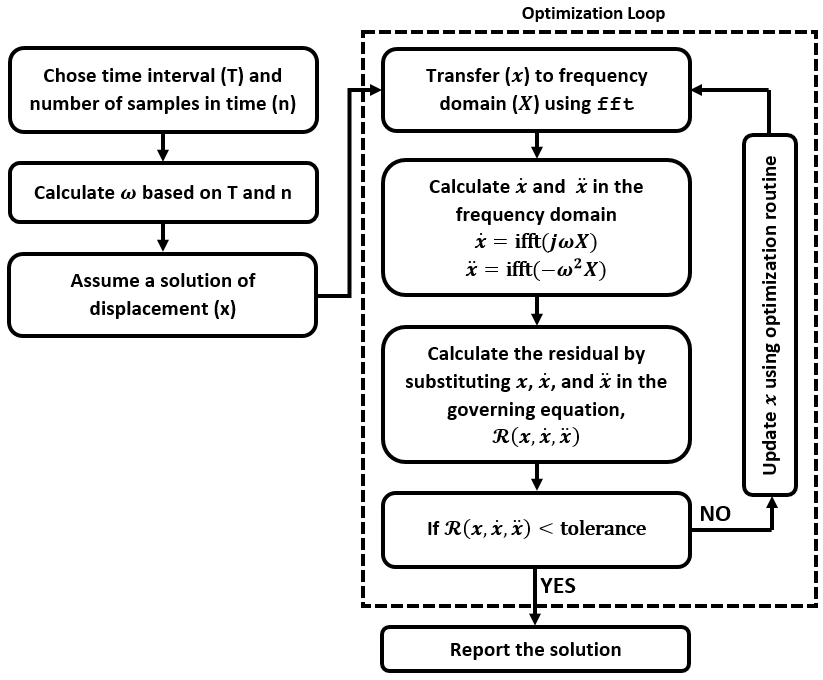
\includegraphics[height=9.00cm]{figure/minimize_residual.png}
	\caption{Flowchart for numerical approach.}
	\label{fig:flowchart}
\end{figure}

To transfer the time domain data for frequency domain we use \texttt{numpy.fft.fft} function and for converting the frequency domain data back to time domain we used \texttt{numpy.fft.ifft}. We sampled the frequency domain using $19$ points. The initial guess for displacement is selected as a vector of ones, \texttt{numpy.ones}. It should be noted that this is a vector of displacement in time. The minimization of residual is done using python \texttt{scipy.optimize.minimize} function using \texttt{SLSQP} method. This process is shown in Figure \ref{fig:flowchart}.

This process can be summarized in the following bullet points

\begin{itemize}

\item An initial guess for response in time domain for a particular time period discretized in required number of samples is made. In general, this assumed solution is zero values (not necessarily).
\item The above initial conditions are then transformed into frequency domain. 
\item Using the properties of fourier series, obtain the derivatives of the responses.
\item Transform the derivatives back into time domain and substitute into the equations of motion.
\item Check if the harmonics are balanced, by minimizing the cost function of the residuals from the equations of motion. 
\item Re-iterate until minimization algorithm meets the convergence criteria tolerance.
\item An initial guess for response in time domain.
\item Transform the initial guess into frequency domain. 
\item Obtain the derivatives of the responses in the frequency domain.
\item Transform the derivatives back into time domain
\item Minimizing the cost function of the residuals from the equations of motion 
\item Re-iterate until minimization algorithm is below it's convergence criteria tolerance.
\end{itemize}

To verify the result of HB method, we used numerical integration to calculate the solution of Equation \eqref{eq:GE}. It should be noted that HB is capable of capturing the steady-state response of the system. Therefore, it is required to let the transient response of the time integration to die of before comparing the results. These are shown in next section.

% ===================================================================
\section{Demonstration Results}
In this section, we apply the method of harmonic balance to different linear and non-linear problems. For the cases where analytical results are not available, we use numerical time integration to verify the results where it shows a good comparison. It should be noted that since the harmonic balance method is used to calculate the limit cycle oscillations of the system. Therefore, it is needed to let the transient part of time integration to die out. Only after this point, the two results match.

% -------------------------------------------------------------------
\subsection{Linear MCK System}
For the first demonstration case we looked at the forced linear damped oscillation of a single degree of freedom system. The governing equation is defined in Equation \eqref{eq:1GE}

\begin{equation}\label{eq:1GE}
	\ddot{x} + \dot{x} + x = \sin 2t
\end{equation}

This equation has a closed form solution that we can use to verify the harmonic balance result. The solution for Equation \eqref{eq:1GE} is calculated as

\begin{equation}
	x(t) = -0.23 \sin 2t - 0.15 \cos 2t
\end{equation}

The comparison between the HB and analytical result for Equation \eqref{eq:1GE} is shown in Figure \ref{fig:R1} for different number of harmonics in HB method. As can be seen here, the HB results matches perfectly with analytical solution of the system.

\begin{figure}[H]
	\centering
	\begin{subfigure}[h]{8.0 cm}
		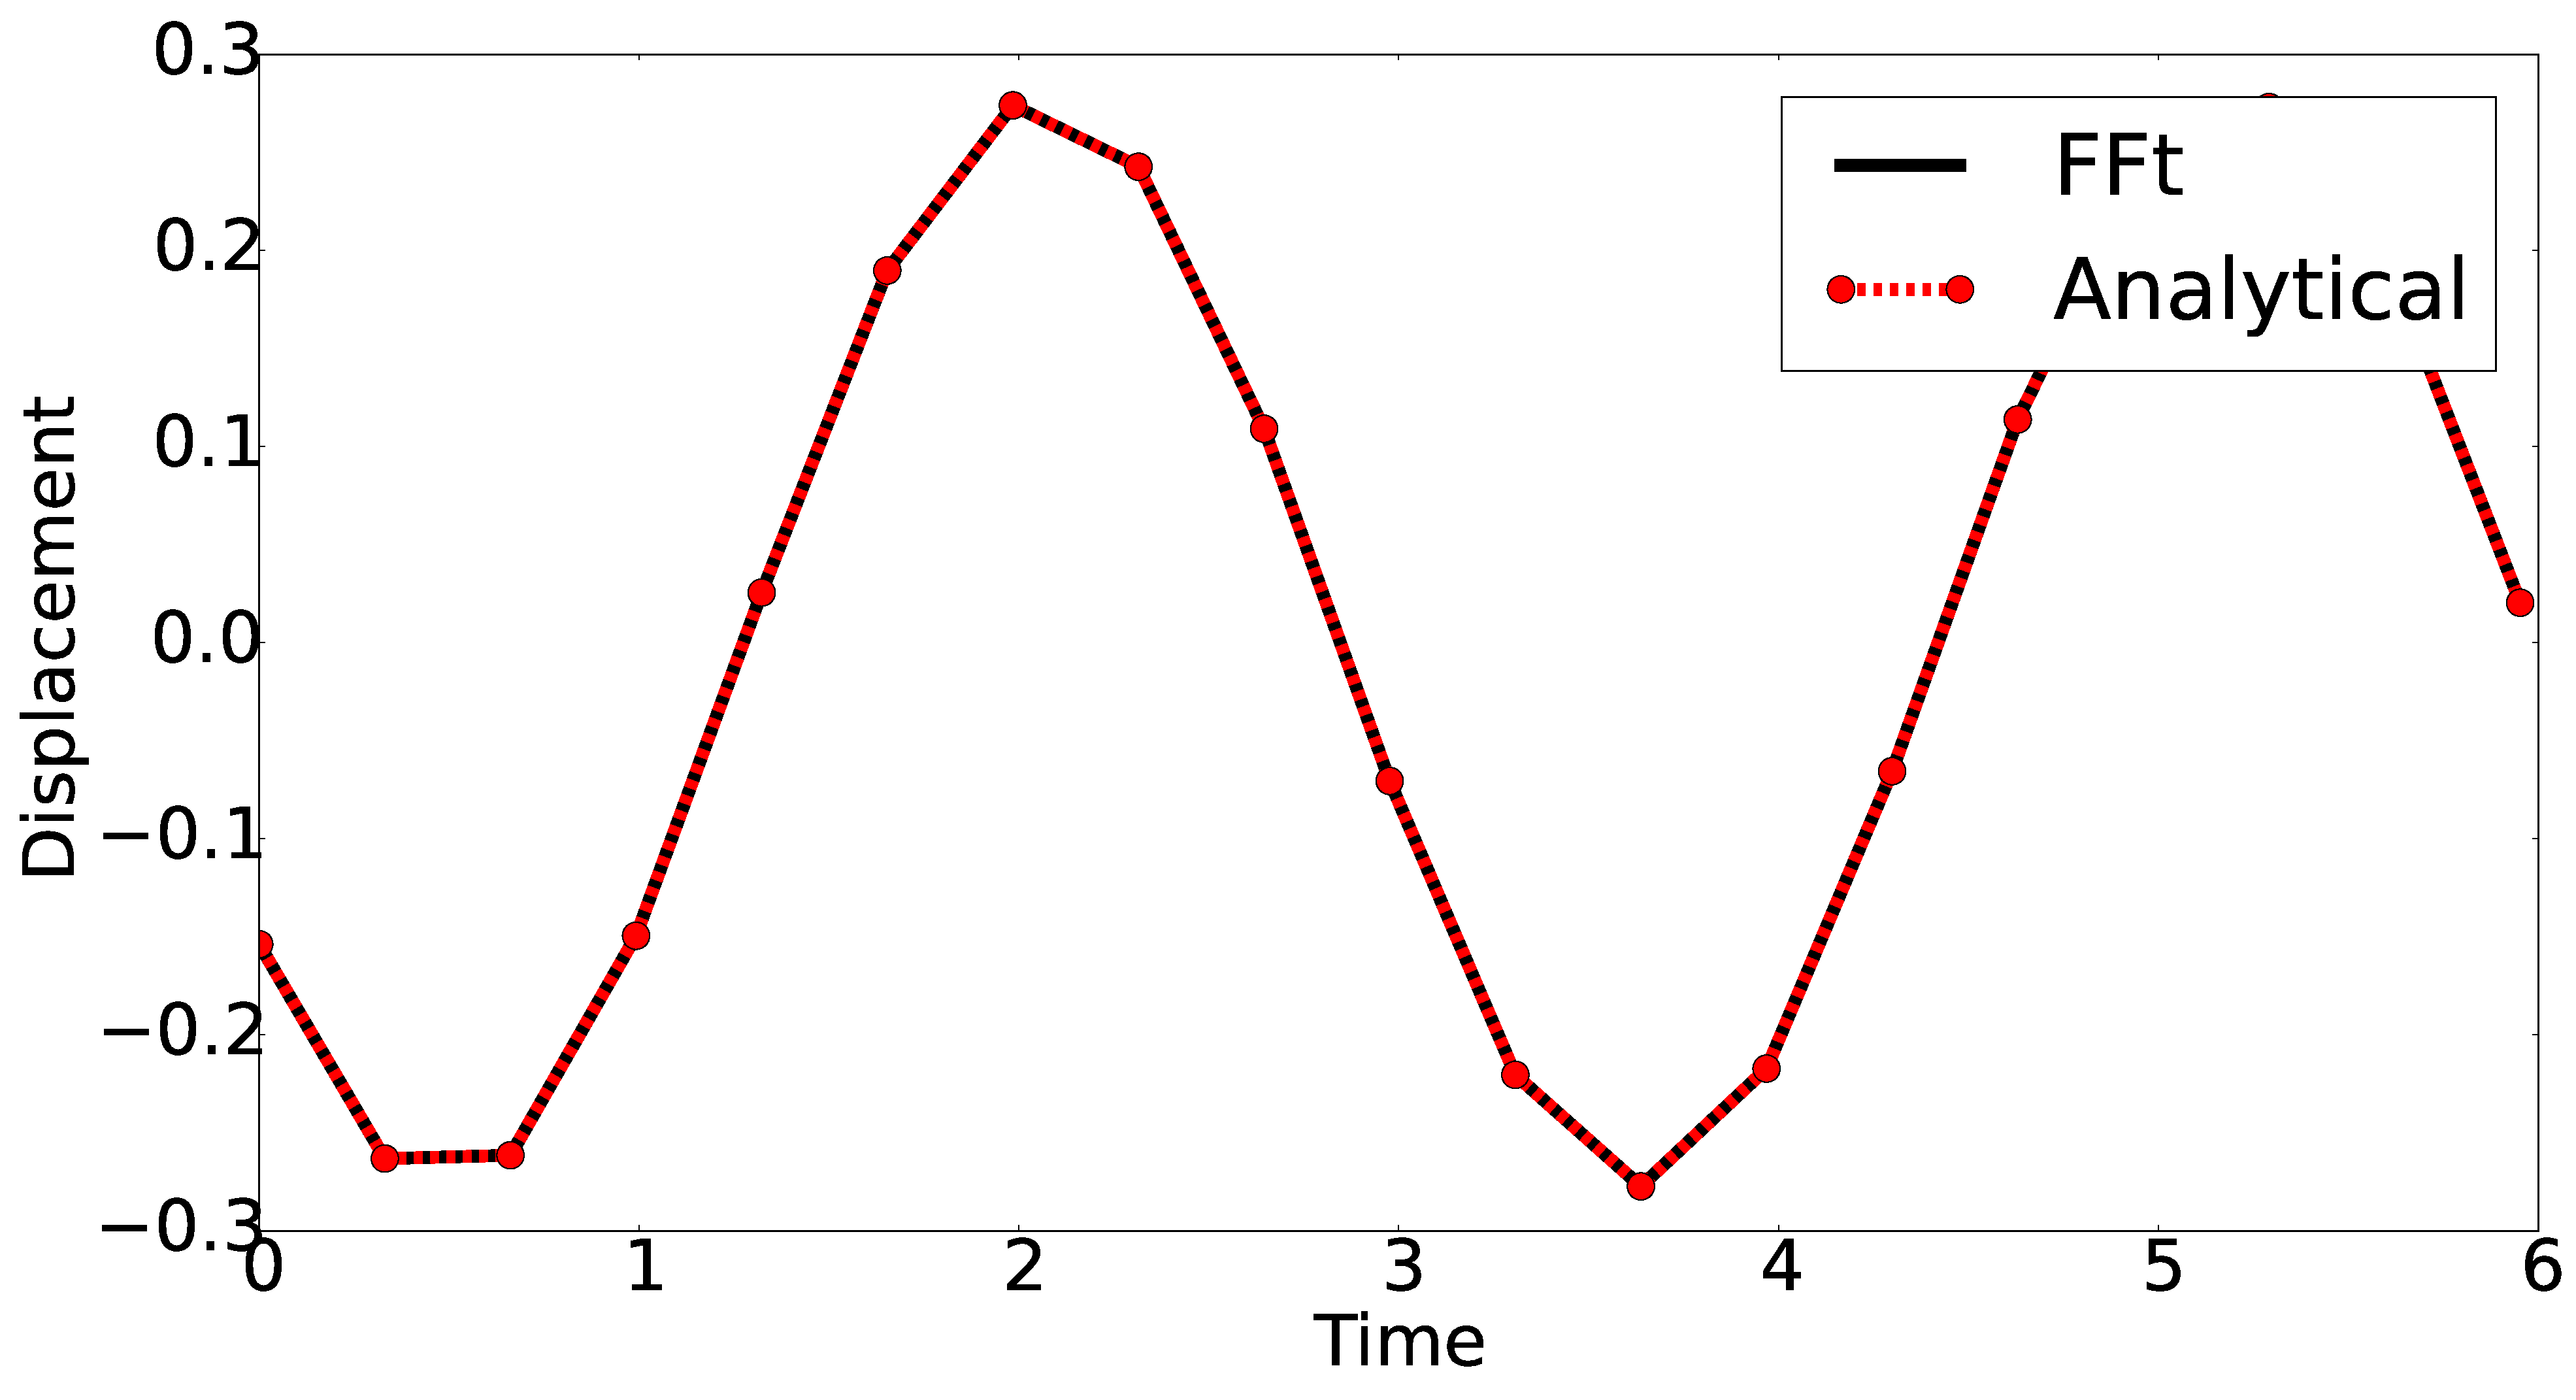
\includegraphics[width=8.0 cm]{figure/1N19.eps}
		\caption{n = 19}
	\end{subfigure}
	\begin{subfigure}[h]{8.0 cm}
        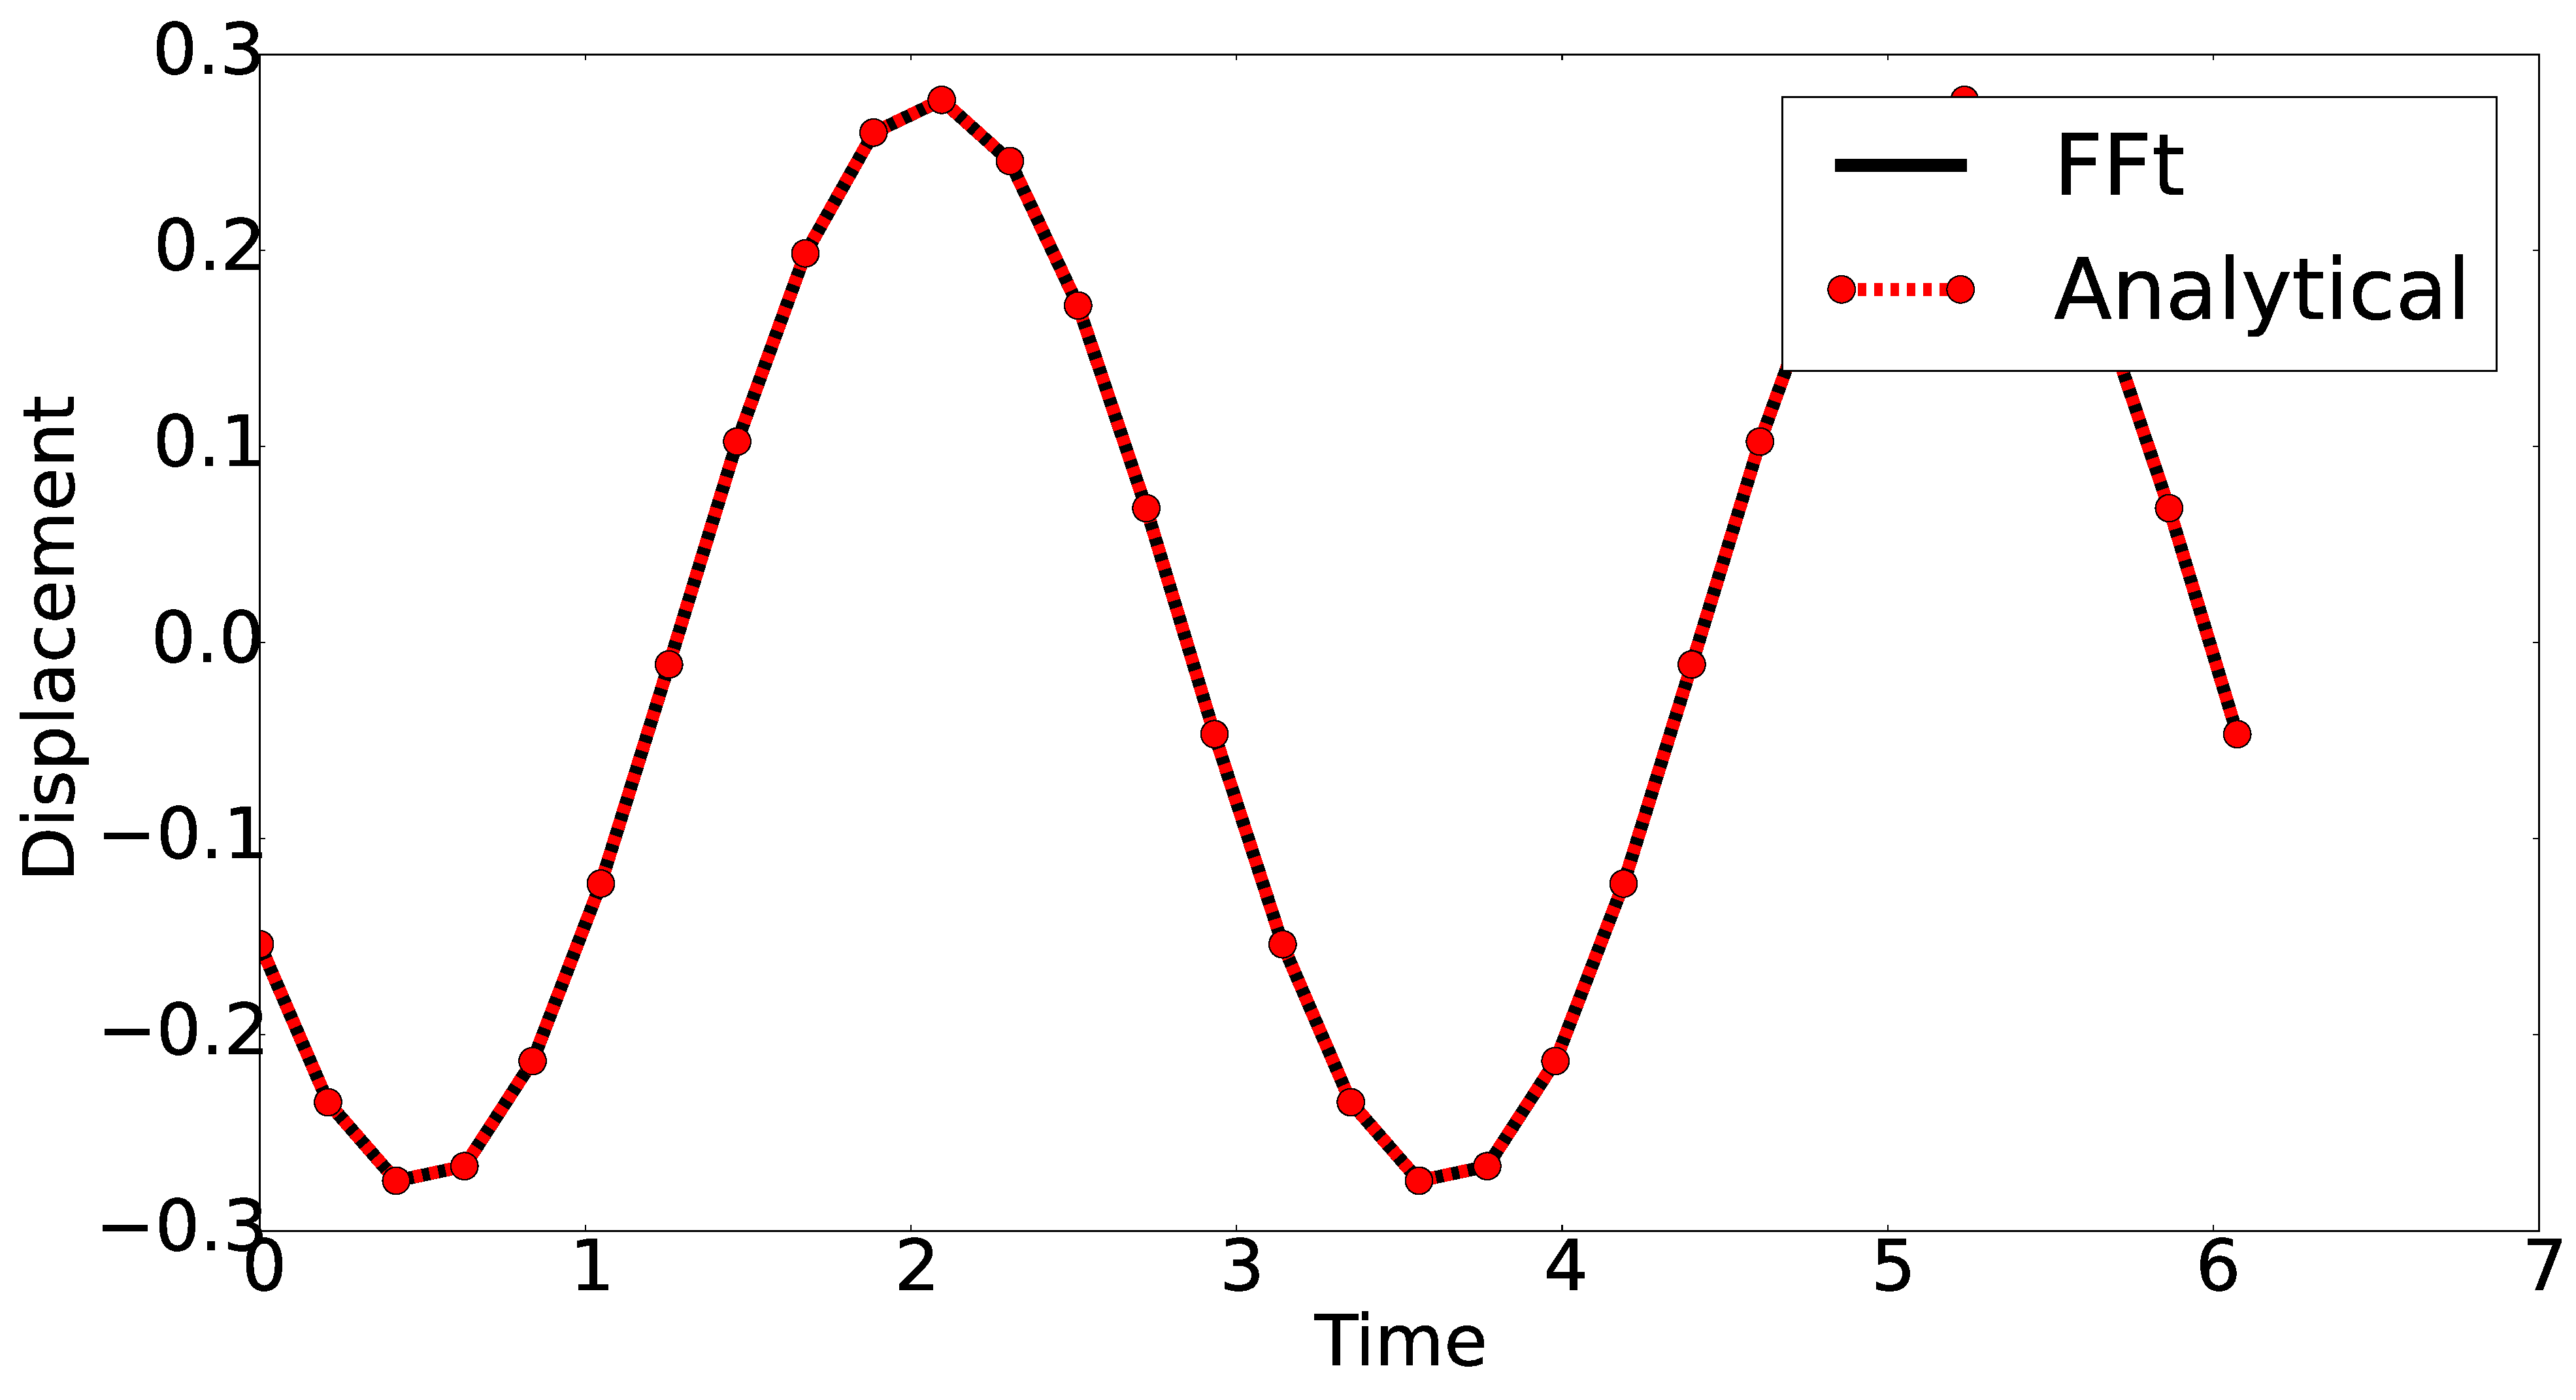
\includegraphics[width=8.0 cm]{figure/1N30.eps}
		\caption{n = 30}
    \end{subfigure}
    \caption{Comparison between HB and analytical result.}
    \label{fig:R1}
\end{figure}

\begin{figure}[H]
	\centering
	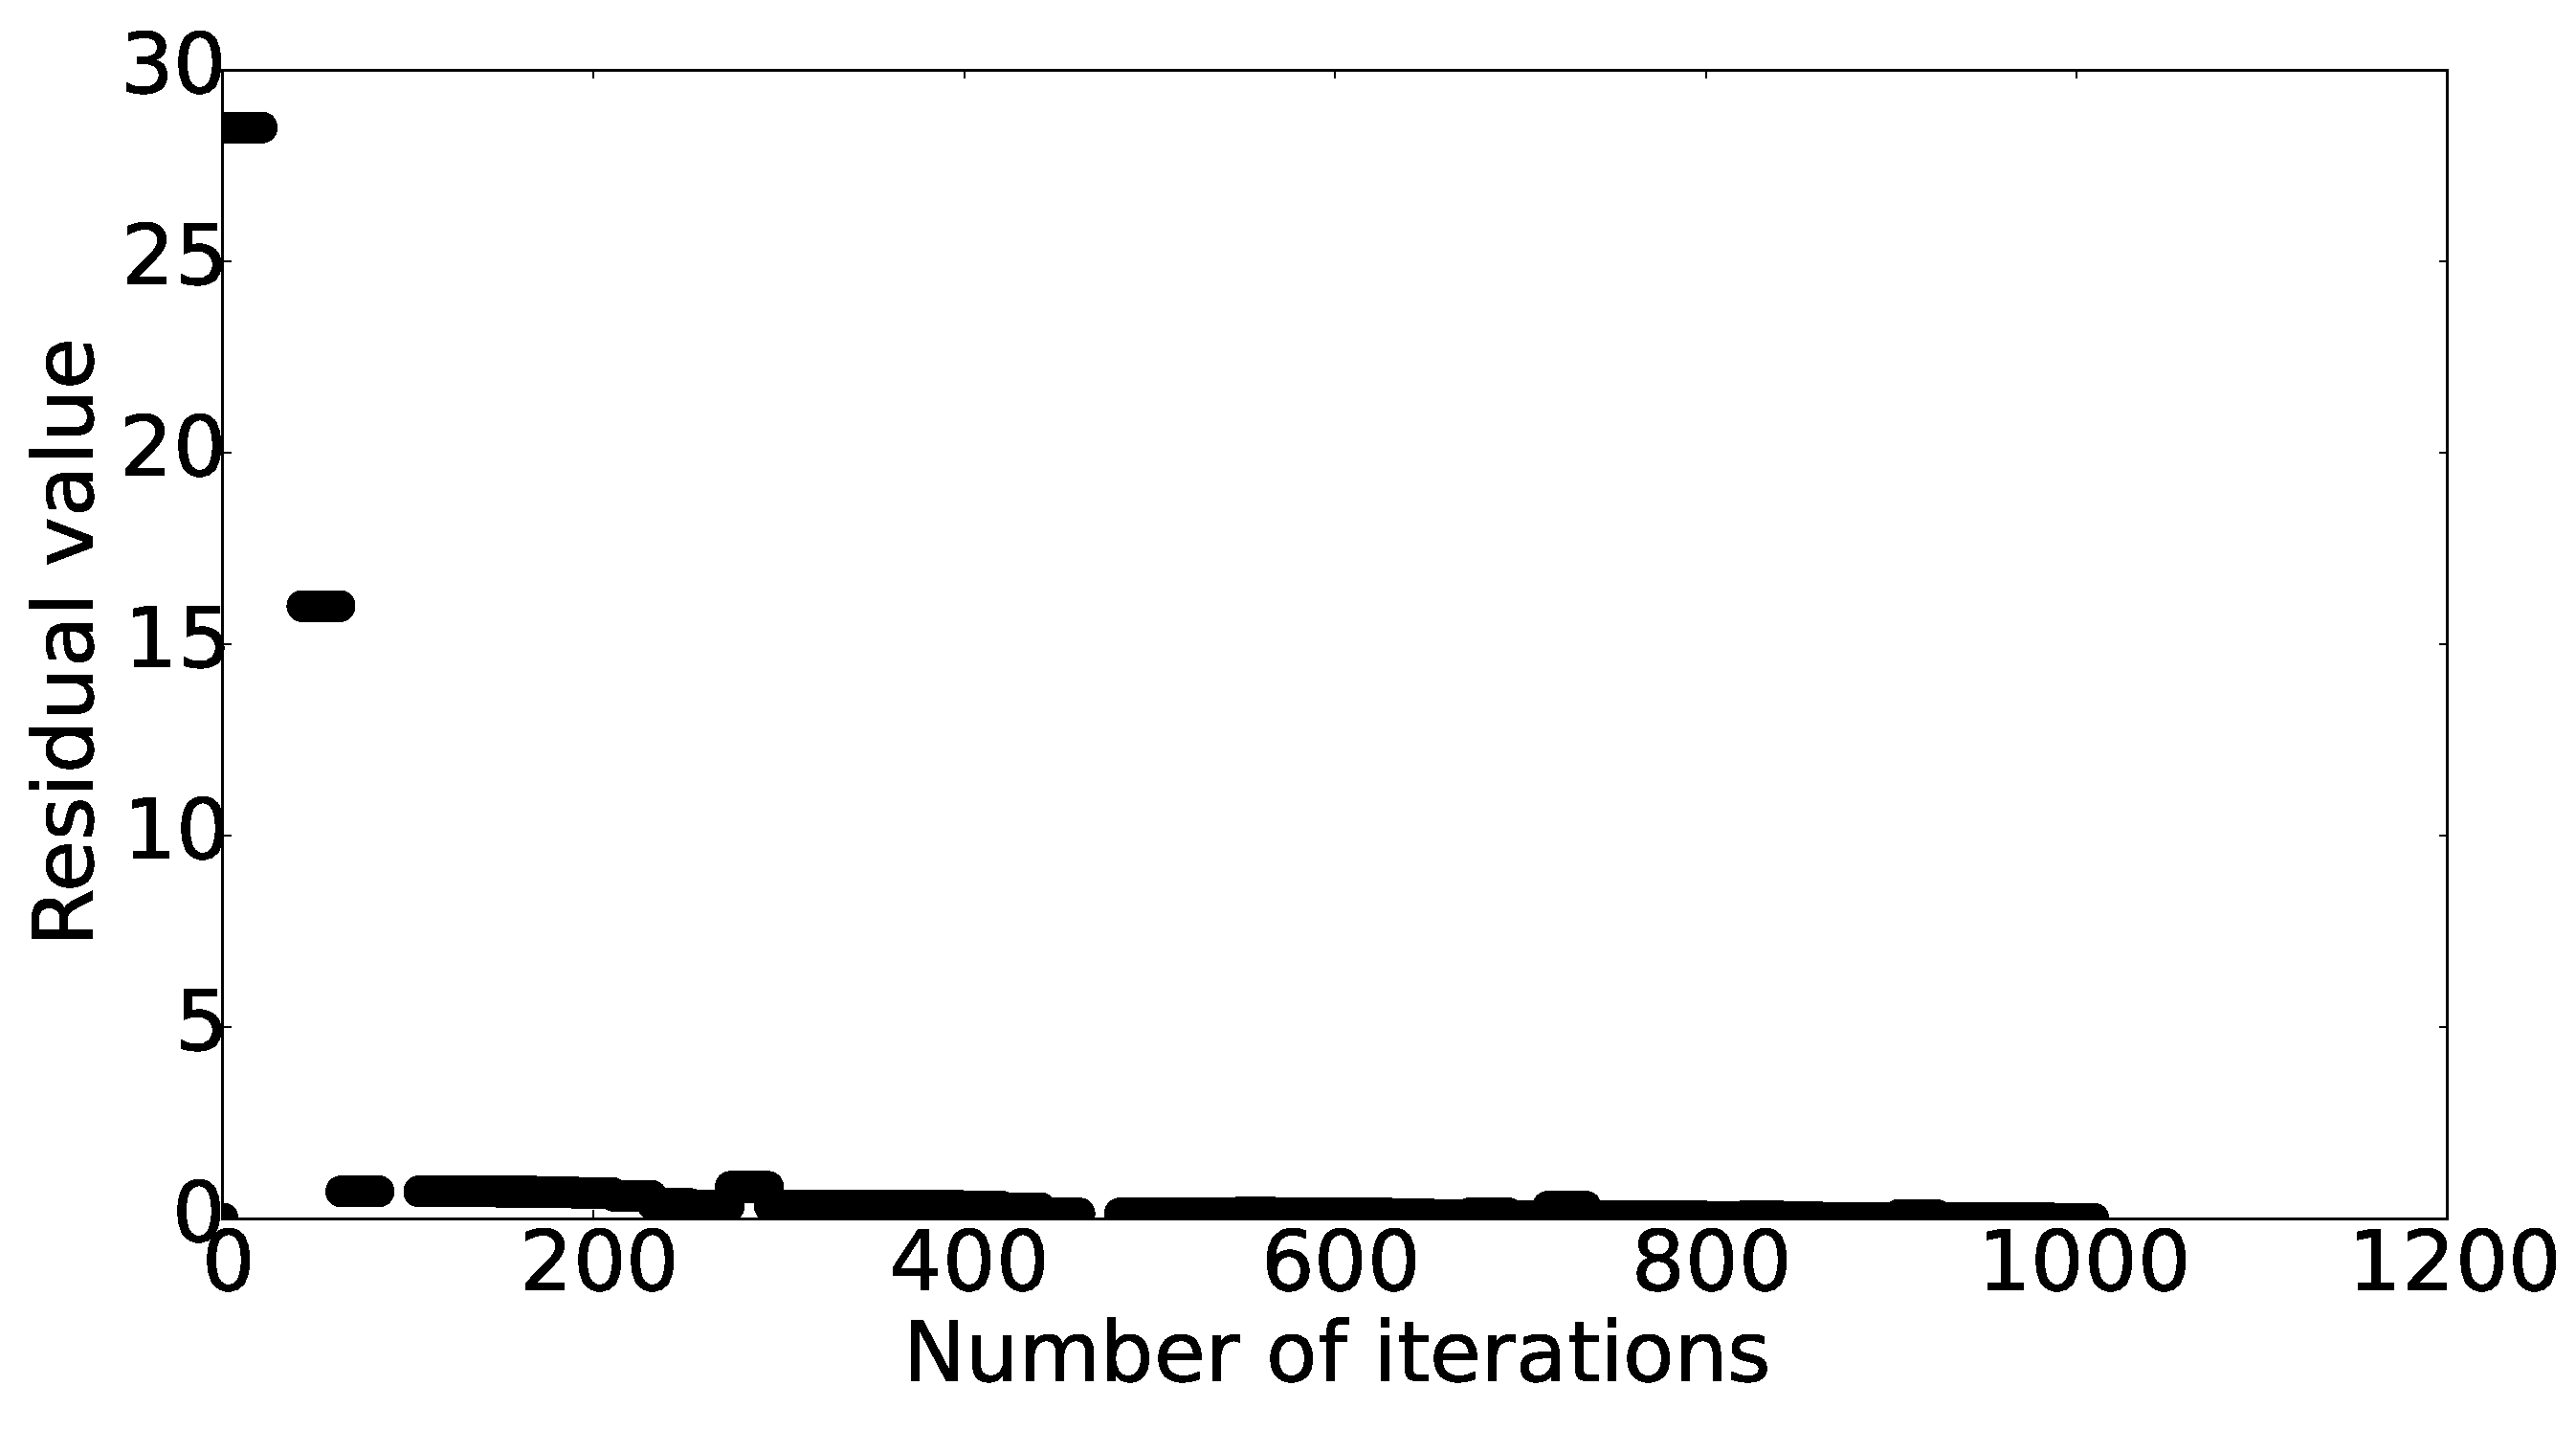
\includegraphics[height=6.00cm]{figure/convergence_study_31.eps}
	\caption{Convergence plot.}
	\label{fig:R1_convergence}
\end{figure}
% -------------------------------------------------------------------

\subsection{Linear System}
The governing equation is defined as
\begin{equation}\label{eq:samGE}
	\ddot{x} + x = \sin 2t
\end{equation}
 
The solution obtained from this equation can be used to compare with  the harmonic balance result. The solution for Equation \eqref{eq:samGE} is calculated as

\begin{equation}
	x(t) = -0.33 \sin 2t
\end{equation}

The following figure\ref{fig:samR1} shows the comparison results between the Harmonic Balance Method and analytical result for Equation \eqref{eq:samGE}. As it can be clearly seen, the Harmonic Balance Method results meets absolutely with analytical solution of the system.

\begin{figure}[H]
	\centering
	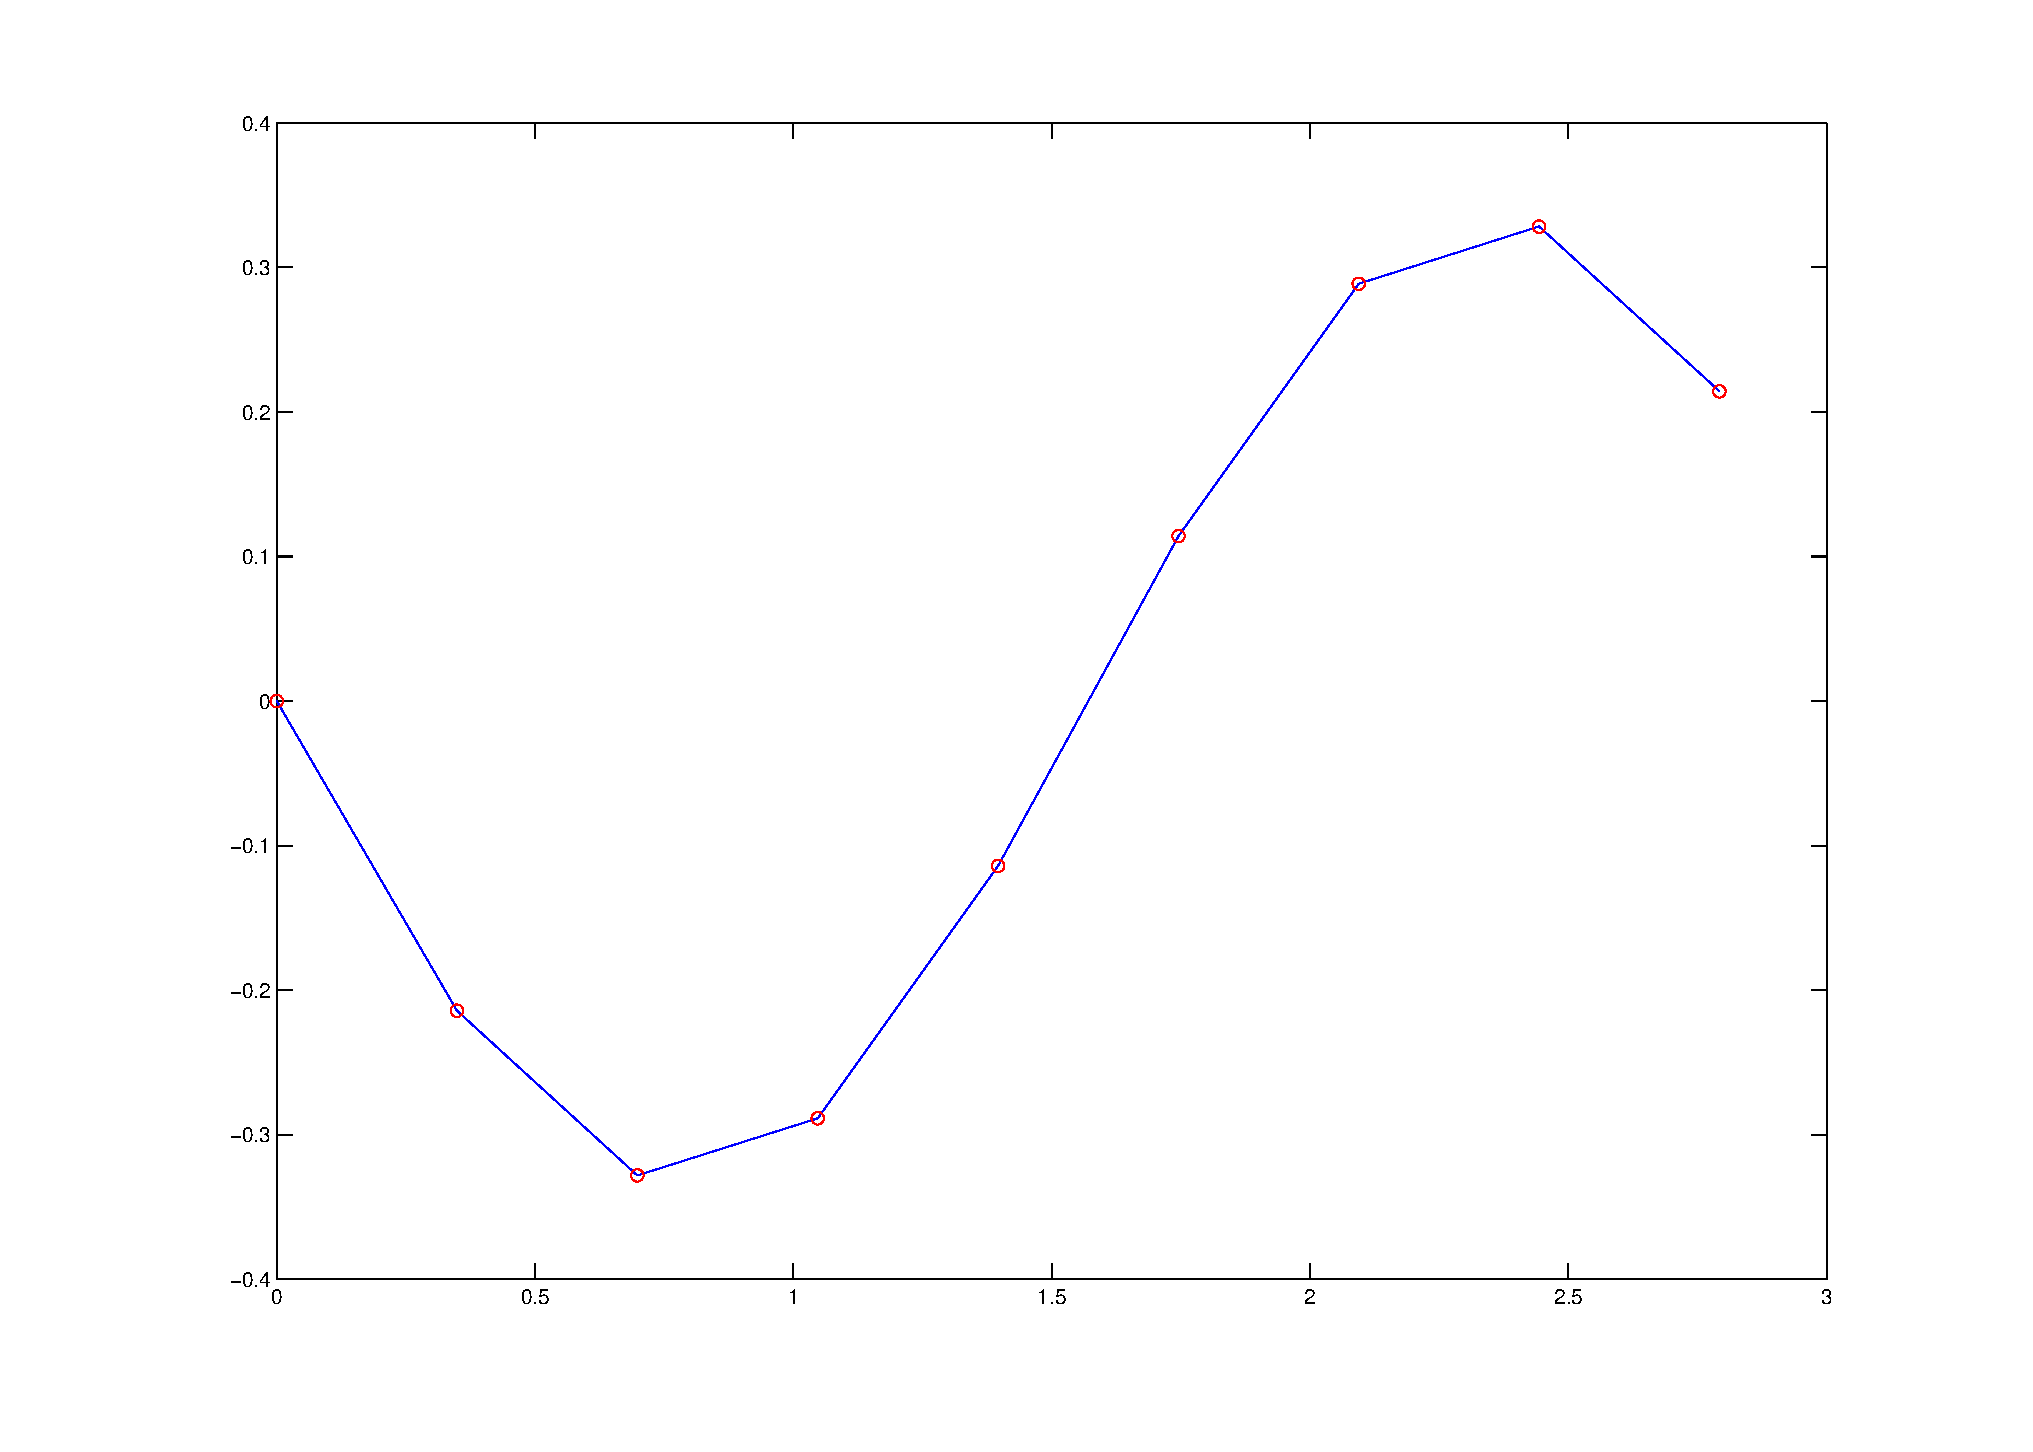
\includegraphics[width=8.0 cm]{figure/fig1.eps}
    \caption{Comparison between Harmonic Balance Method and analytical result.}
    \label{fig:samR1}
\end{figure}
% -------------------------------------------------------------------
\subsection{Nonlinear Oscillator}
For the second demonstration example, we looked at problem 2.45 on page 140 of Applied Nonlinear Dynamics (Nayfeh) book. The governing equation for this problem is shown in Equation \eqref{eq:2GE}

\begin{equation}\label{eq:2GE}
	\ddot{x} + 2 \mu \dot{x} + \frac{g}{R} \sin x - \alpha^2 \sin x \cos x = \sin 2t
\end{equation}

In above equation, we chose $\mu = 0.1$, $g = 9.81$, $R = 1.0$, and $\alpha = 1$. We used \texttt{odeint} function in \texttt{python} for time integration to verify the results of HB method. This is shown in Figure \ref{fig:R2}. As shown here, HB is in good agreement with the numerical solution at both low and high order sampling. The response converges and coincides with analytical solution as the transient part of the solution dies out.

\begin{figure}[H]
	\centering
	\begin{subfigure}[h]{8.0 cm}
		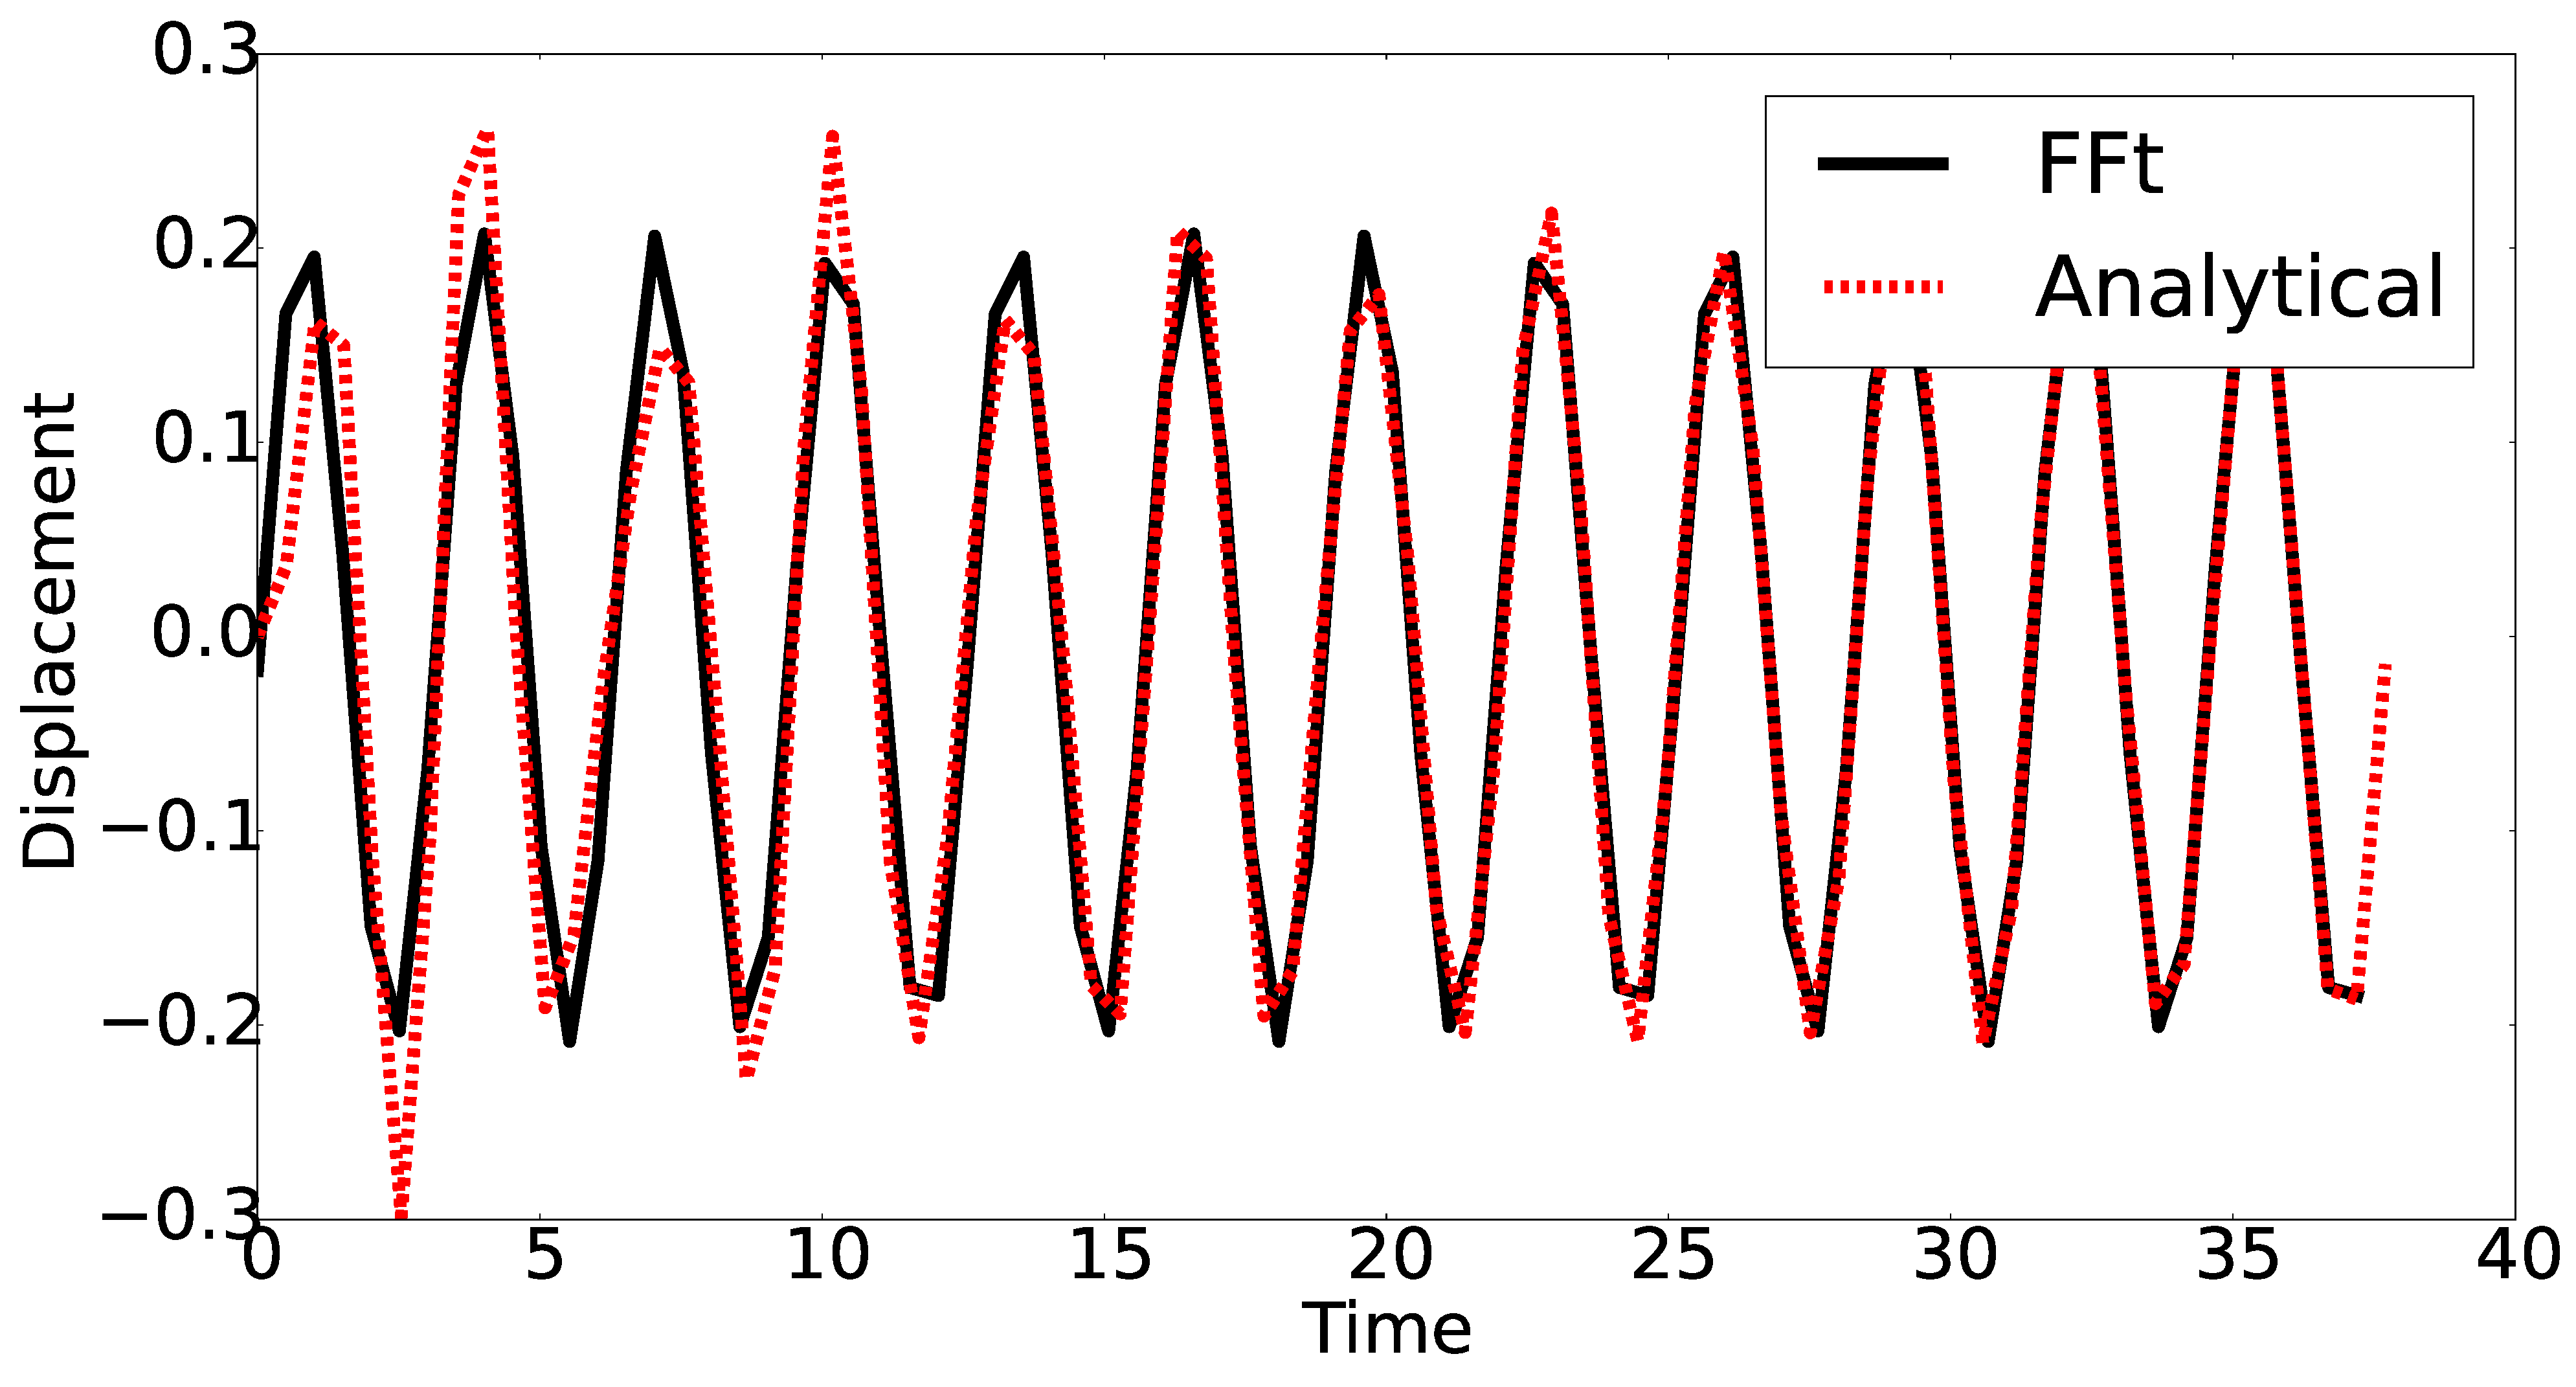
\includegraphics[width=8.0 cm]{figure/2N75.eps}
		\caption{n = 75}
	\end{subfigure}
	\begin{subfigure}[h]{8.0 cm}
        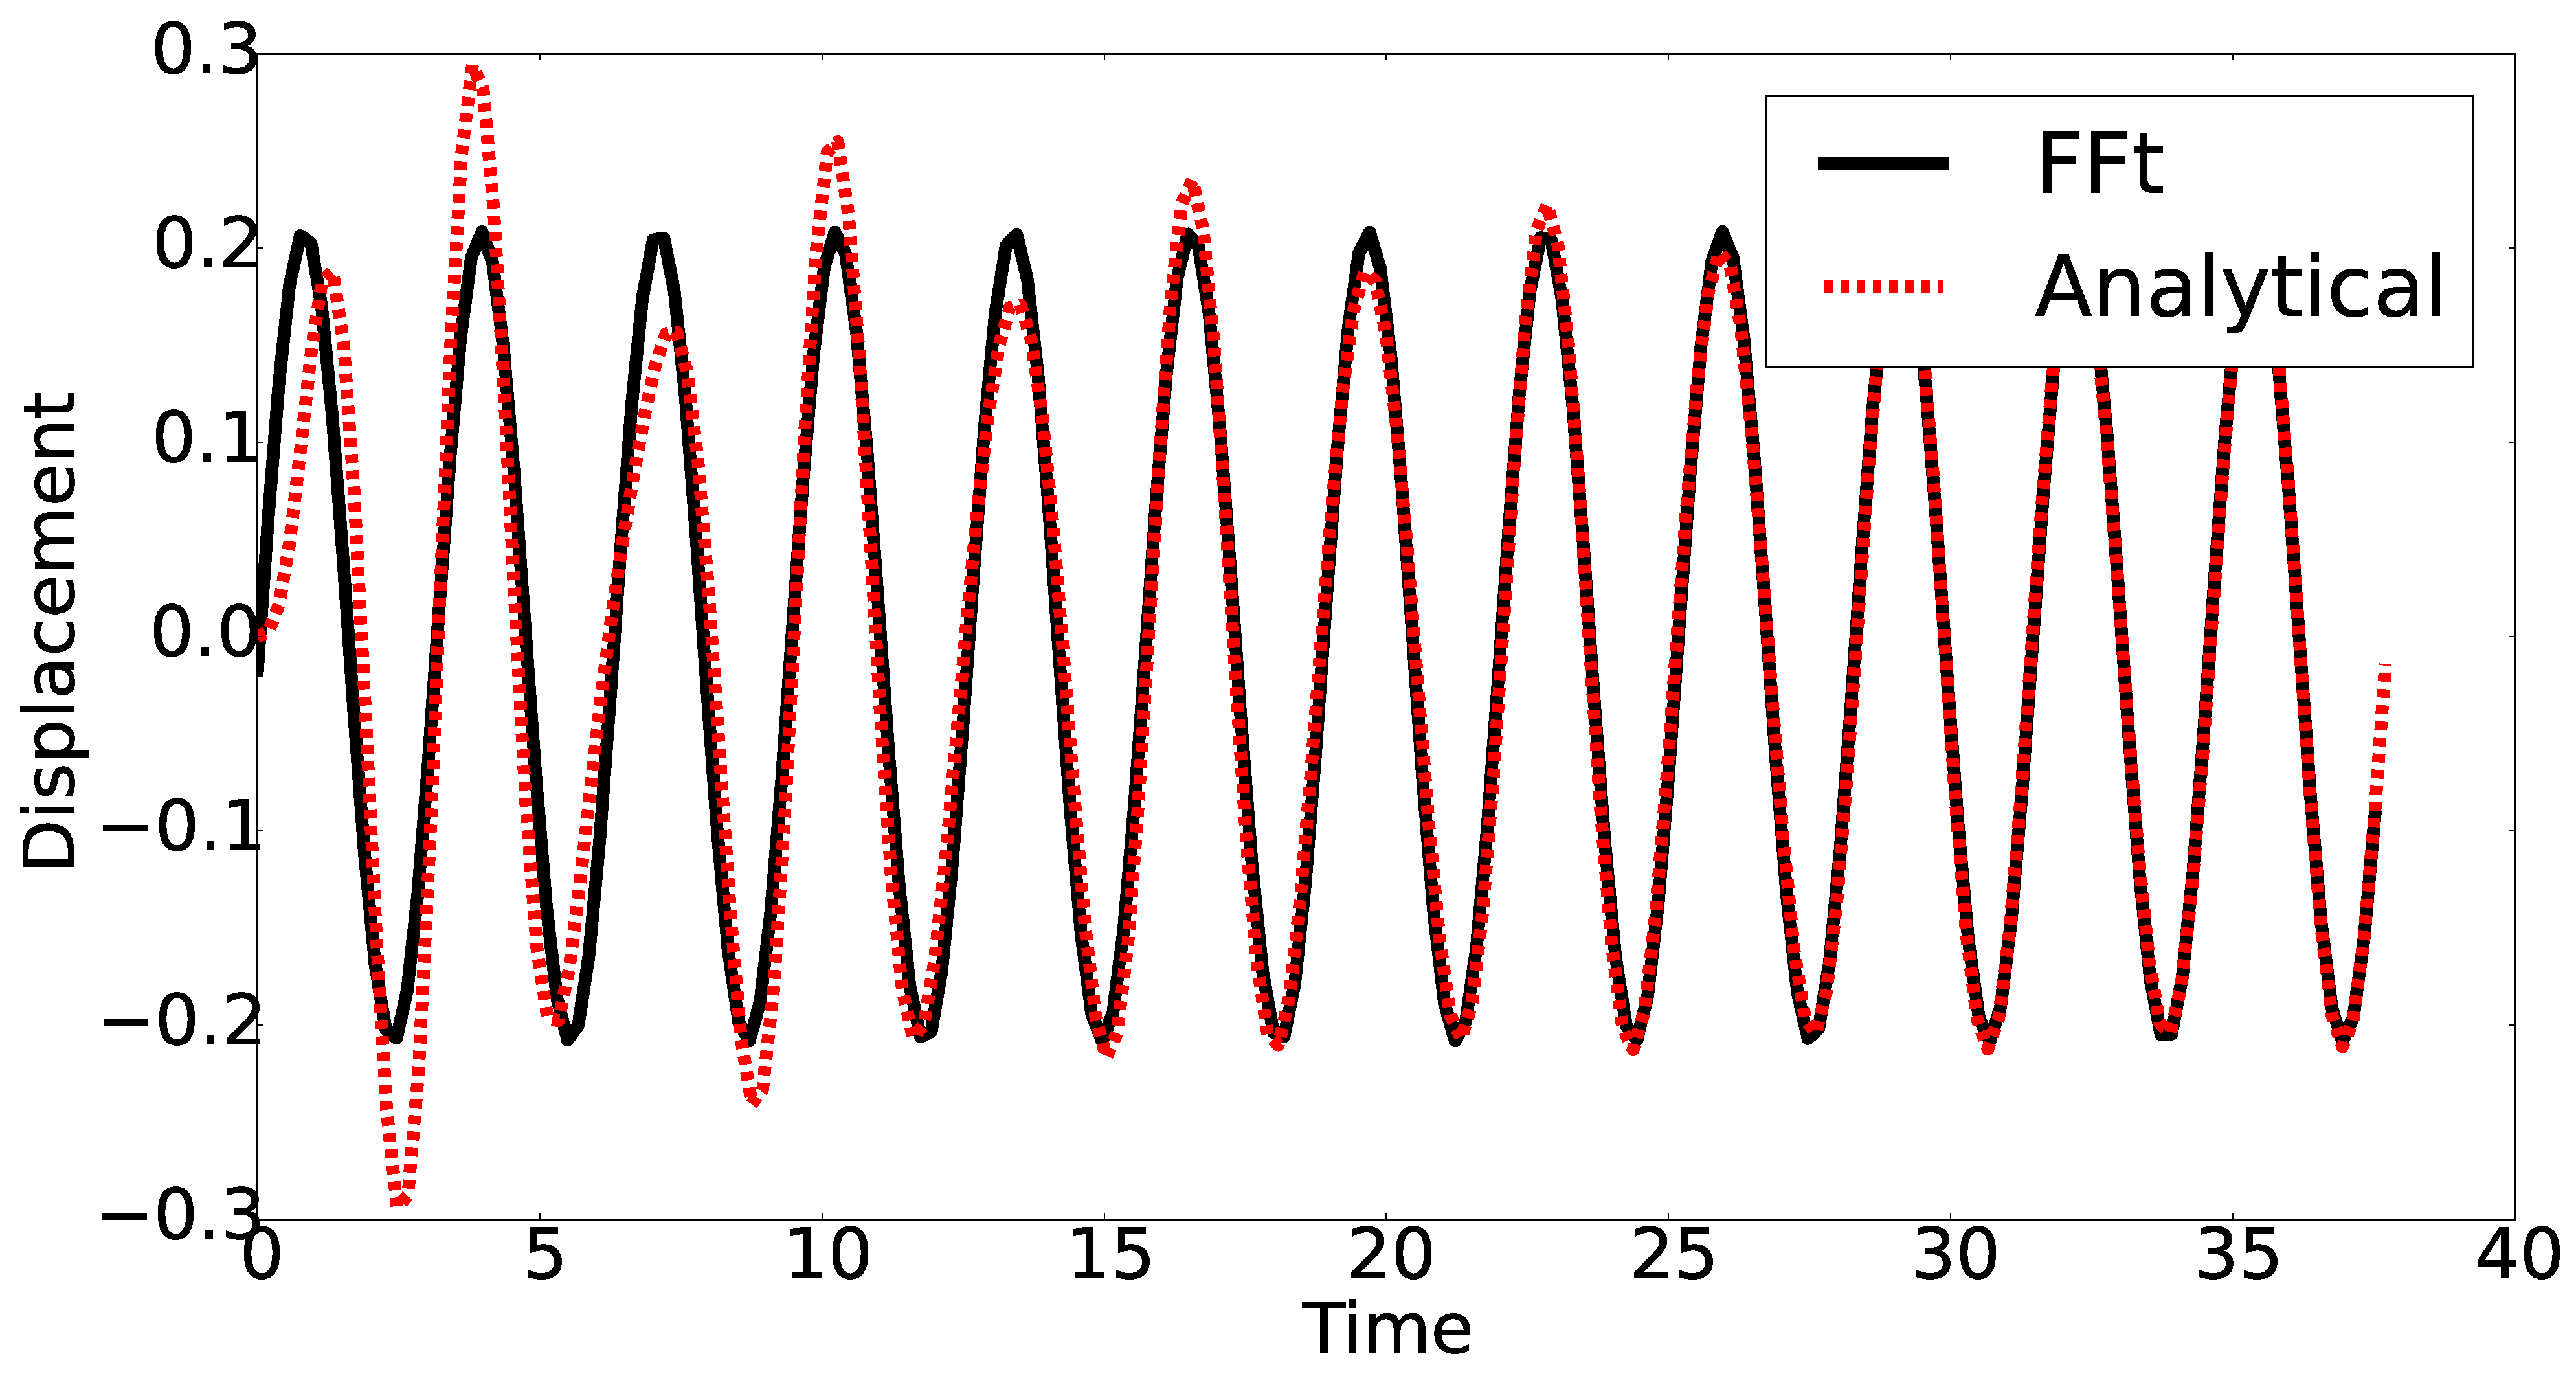
\includegraphics[width=8.0 cm]{figure/2N199.eps}
		\caption{n = 199}
    \end{subfigure}
    \caption{Comparison between HB and analytical result.}
    \label{fig:R2}
\end{figure}

The convergence results for the residual is shown in Figure \ref{fig:R2_convergence}. As can be seen here, the value of residual reaches zero at the end of the optimization process. The flat lines represents the finite difference steps required to calculated the Jacobian.

\begin{figure}[H]
	\centering
	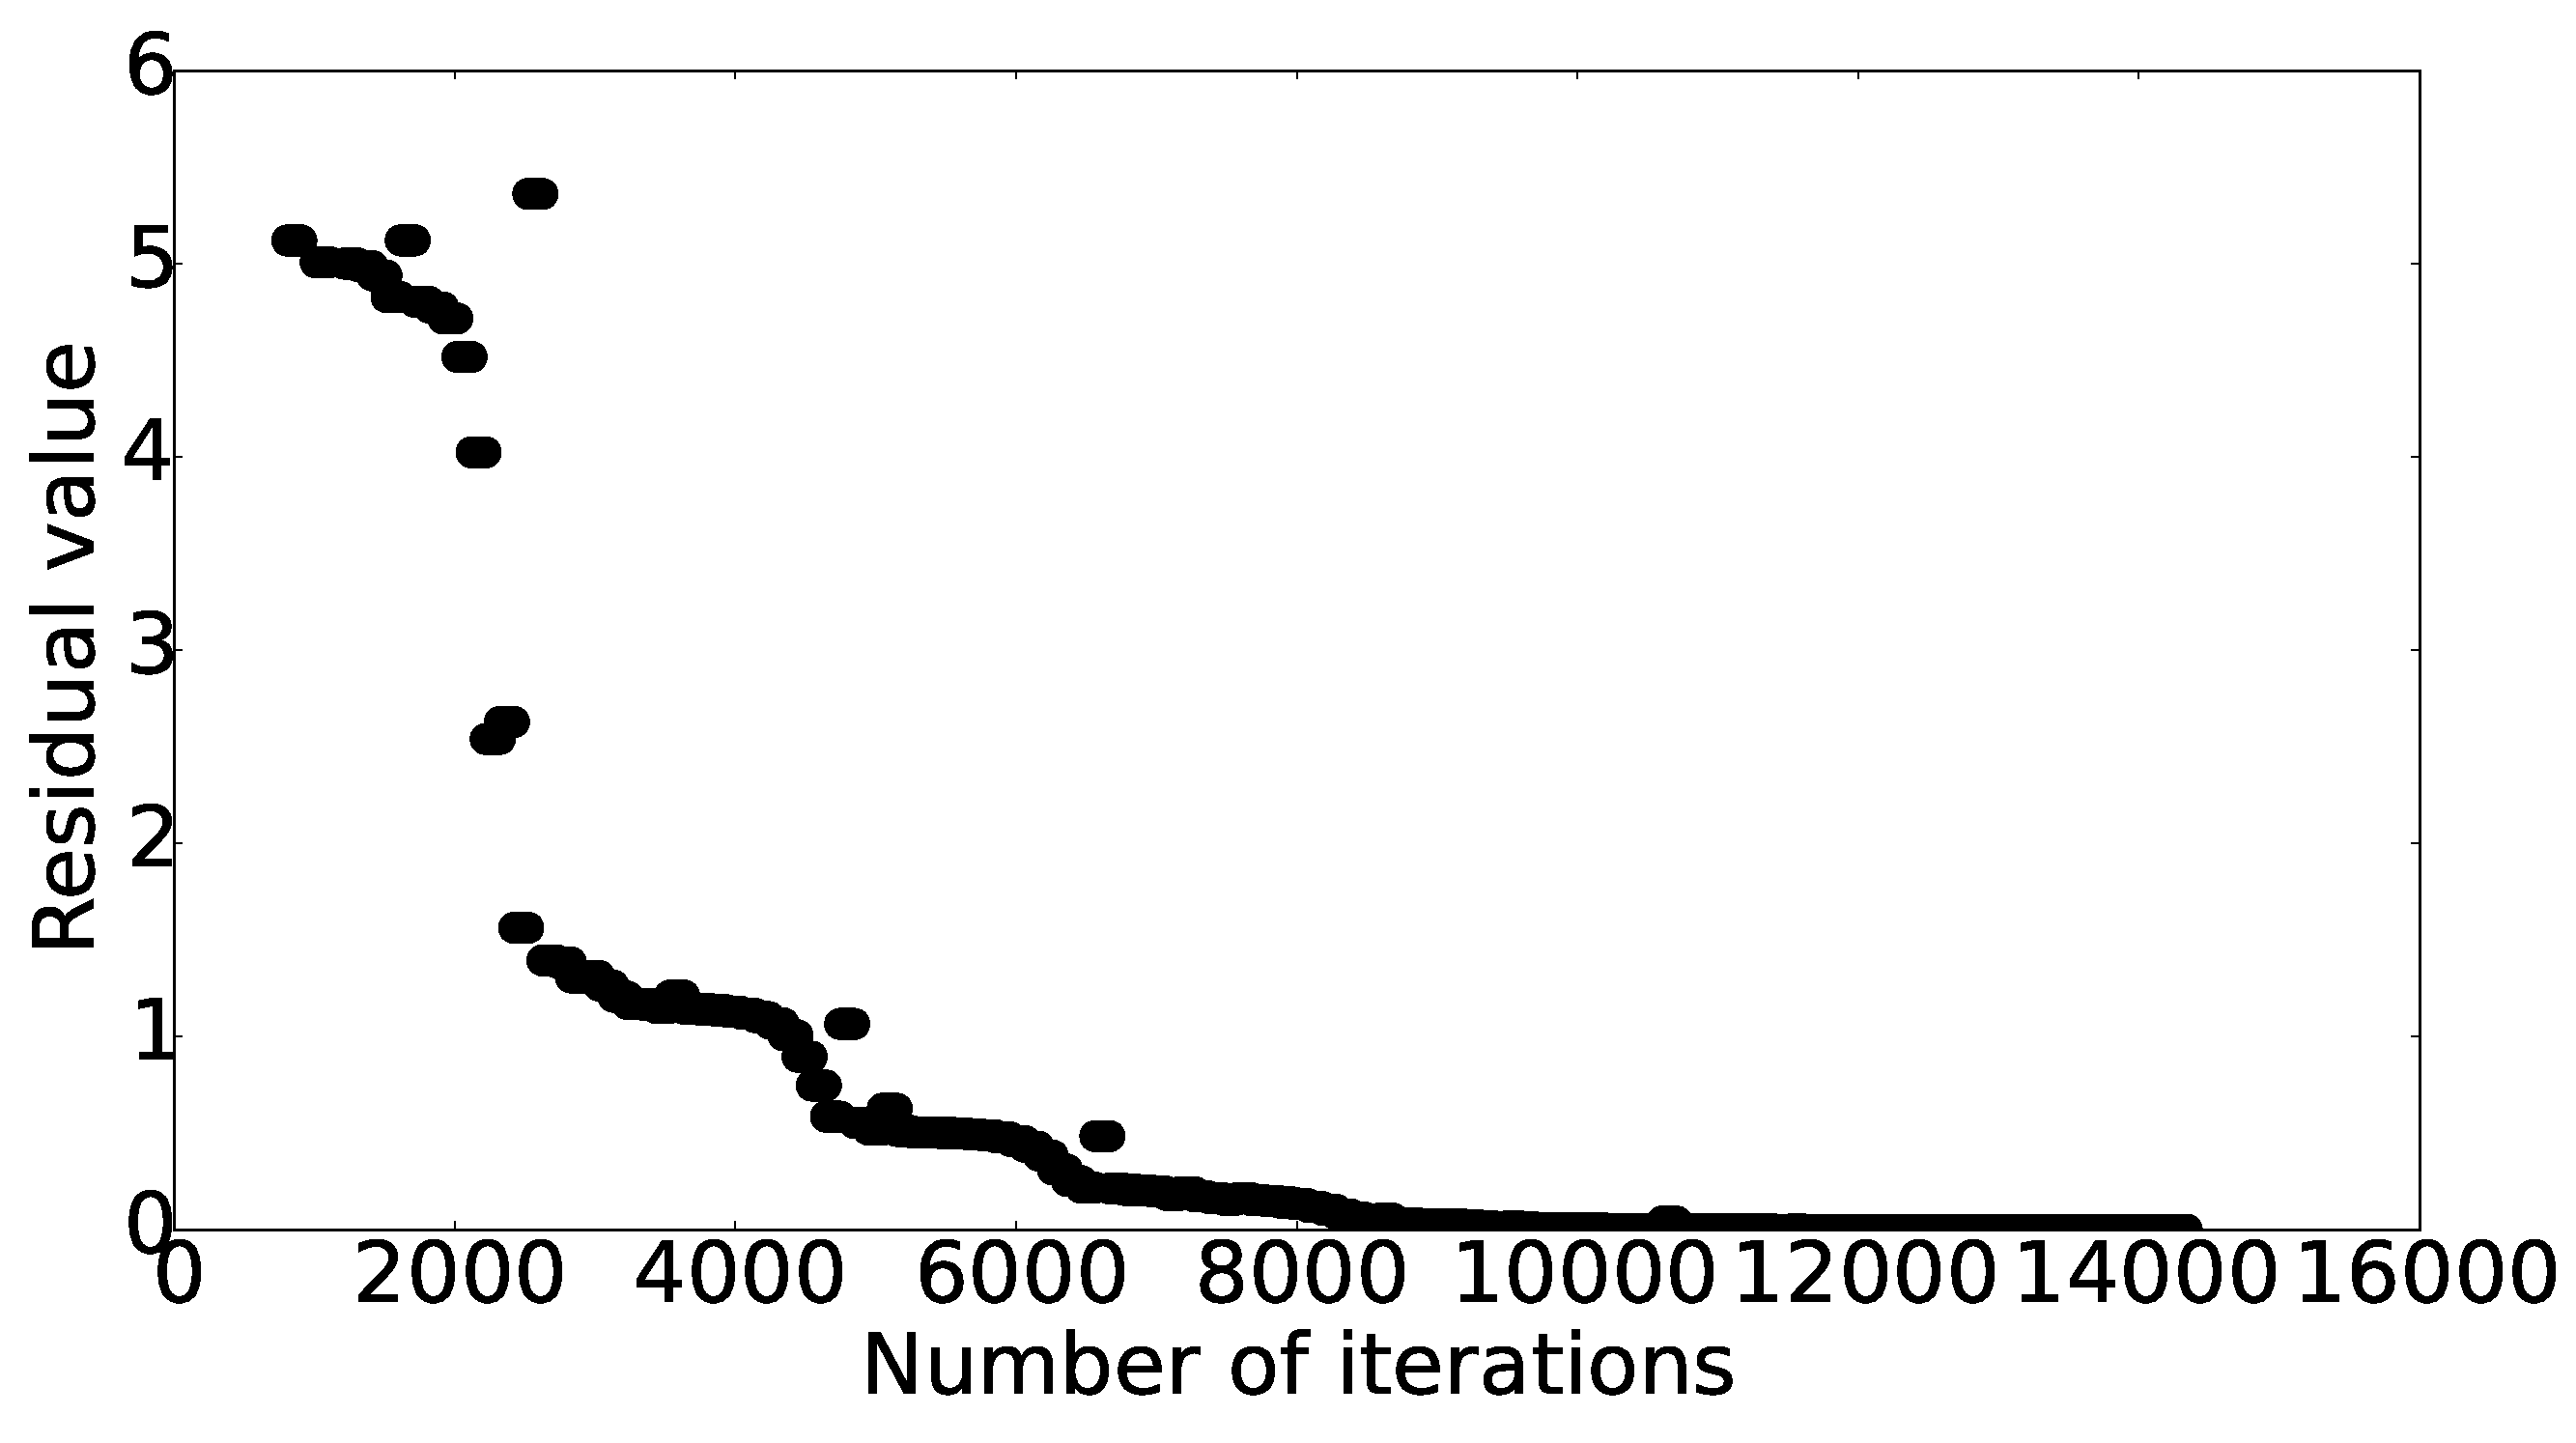
\includegraphics[height=6.00cm]{figure/convergence_study_32.eps}
	\caption{Convergence plot.}
	\label{fig:R2_convergence}
\end{figure}

% -------------------------------------------------------------------
\subsection{Parametrically excited Duffing Oscillator}
We looked at the applicability of HB in handling the nonlinear, force, parametrically excited Duffing oscillator. The governing equation of this system is shown in Equation \eqref{eq:3GE}.

\begin{equation}\label{eq:3GE}
	\ddot{x} + x + \epsilon \left[ 2 \mu \dot{x} + \alpha x^3 + 2 k x \cos \omega t \right] = \sin 2t	
\end{equation}

We chose $\epsilon = 1.0$, $\mu = 1.0$, $\alpha = 1.0$, $k = 1.0$, and $\omega = 2.0$ for the system parameters. Like the previous example, we used time integration to verify the results of HB method as shown in Figure \ref{fig:R3}. As seen here, similar convergence trend is observed for parametrically excited nonlinear oscillating system for different number of harmonics.

\begin{figure}[H]
	\centering
	\begin{subfigure}[h]{8.0 cm}
		
\includegraphics[width=8.0 cm]{figure/3N20.eps}
		\caption{n = 20}
	\end{subfigure}
	\begin{subfigure}[h]{8.0 cm}
        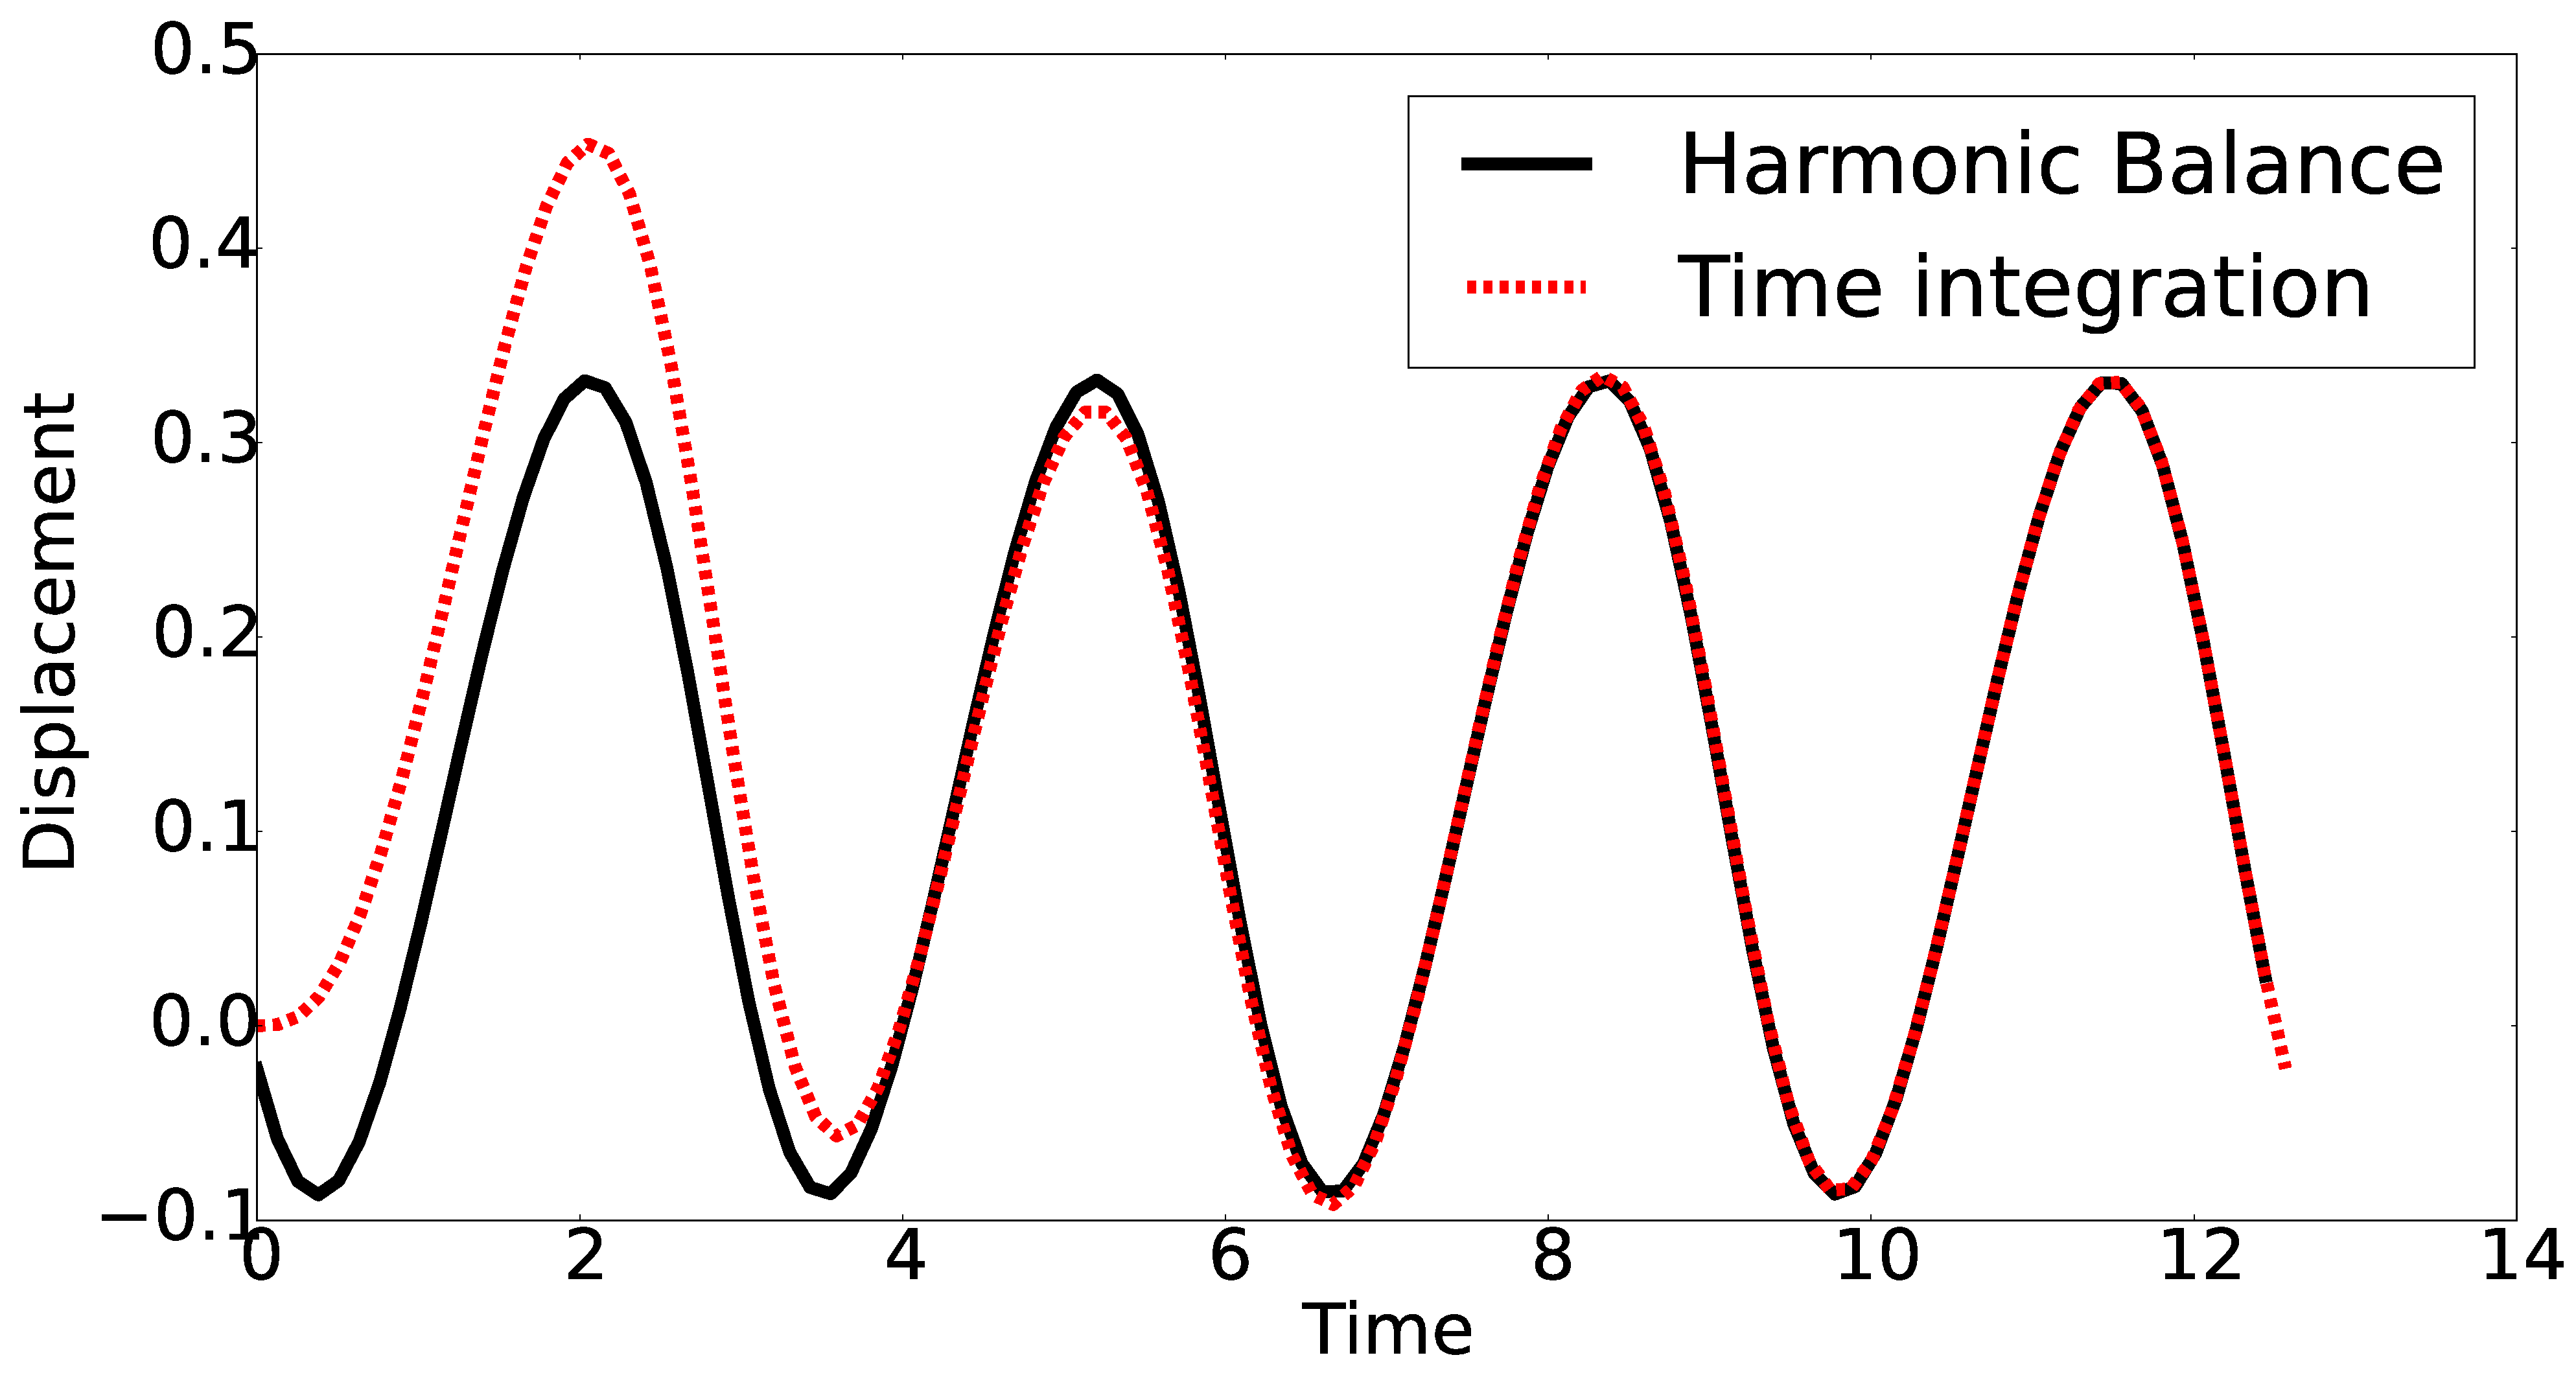
\includegraphics[width=8.0 cm]{figure/3N99.eps}
		\caption{n = 99}
    \end{subfigure}
    \caption{Comparison between HB and analytical result.}
    \label{fig:R3}
\end{figure}

The convergence results for the residual is shown in Figure \ref{fig:R3_convergence}. As can be seen here, the value of residual reaches zero at the end of the optimization process. The flat lines represents the finite difference steps required to calculated the Jacobian.

\begin{figure}[H]
	\centering
	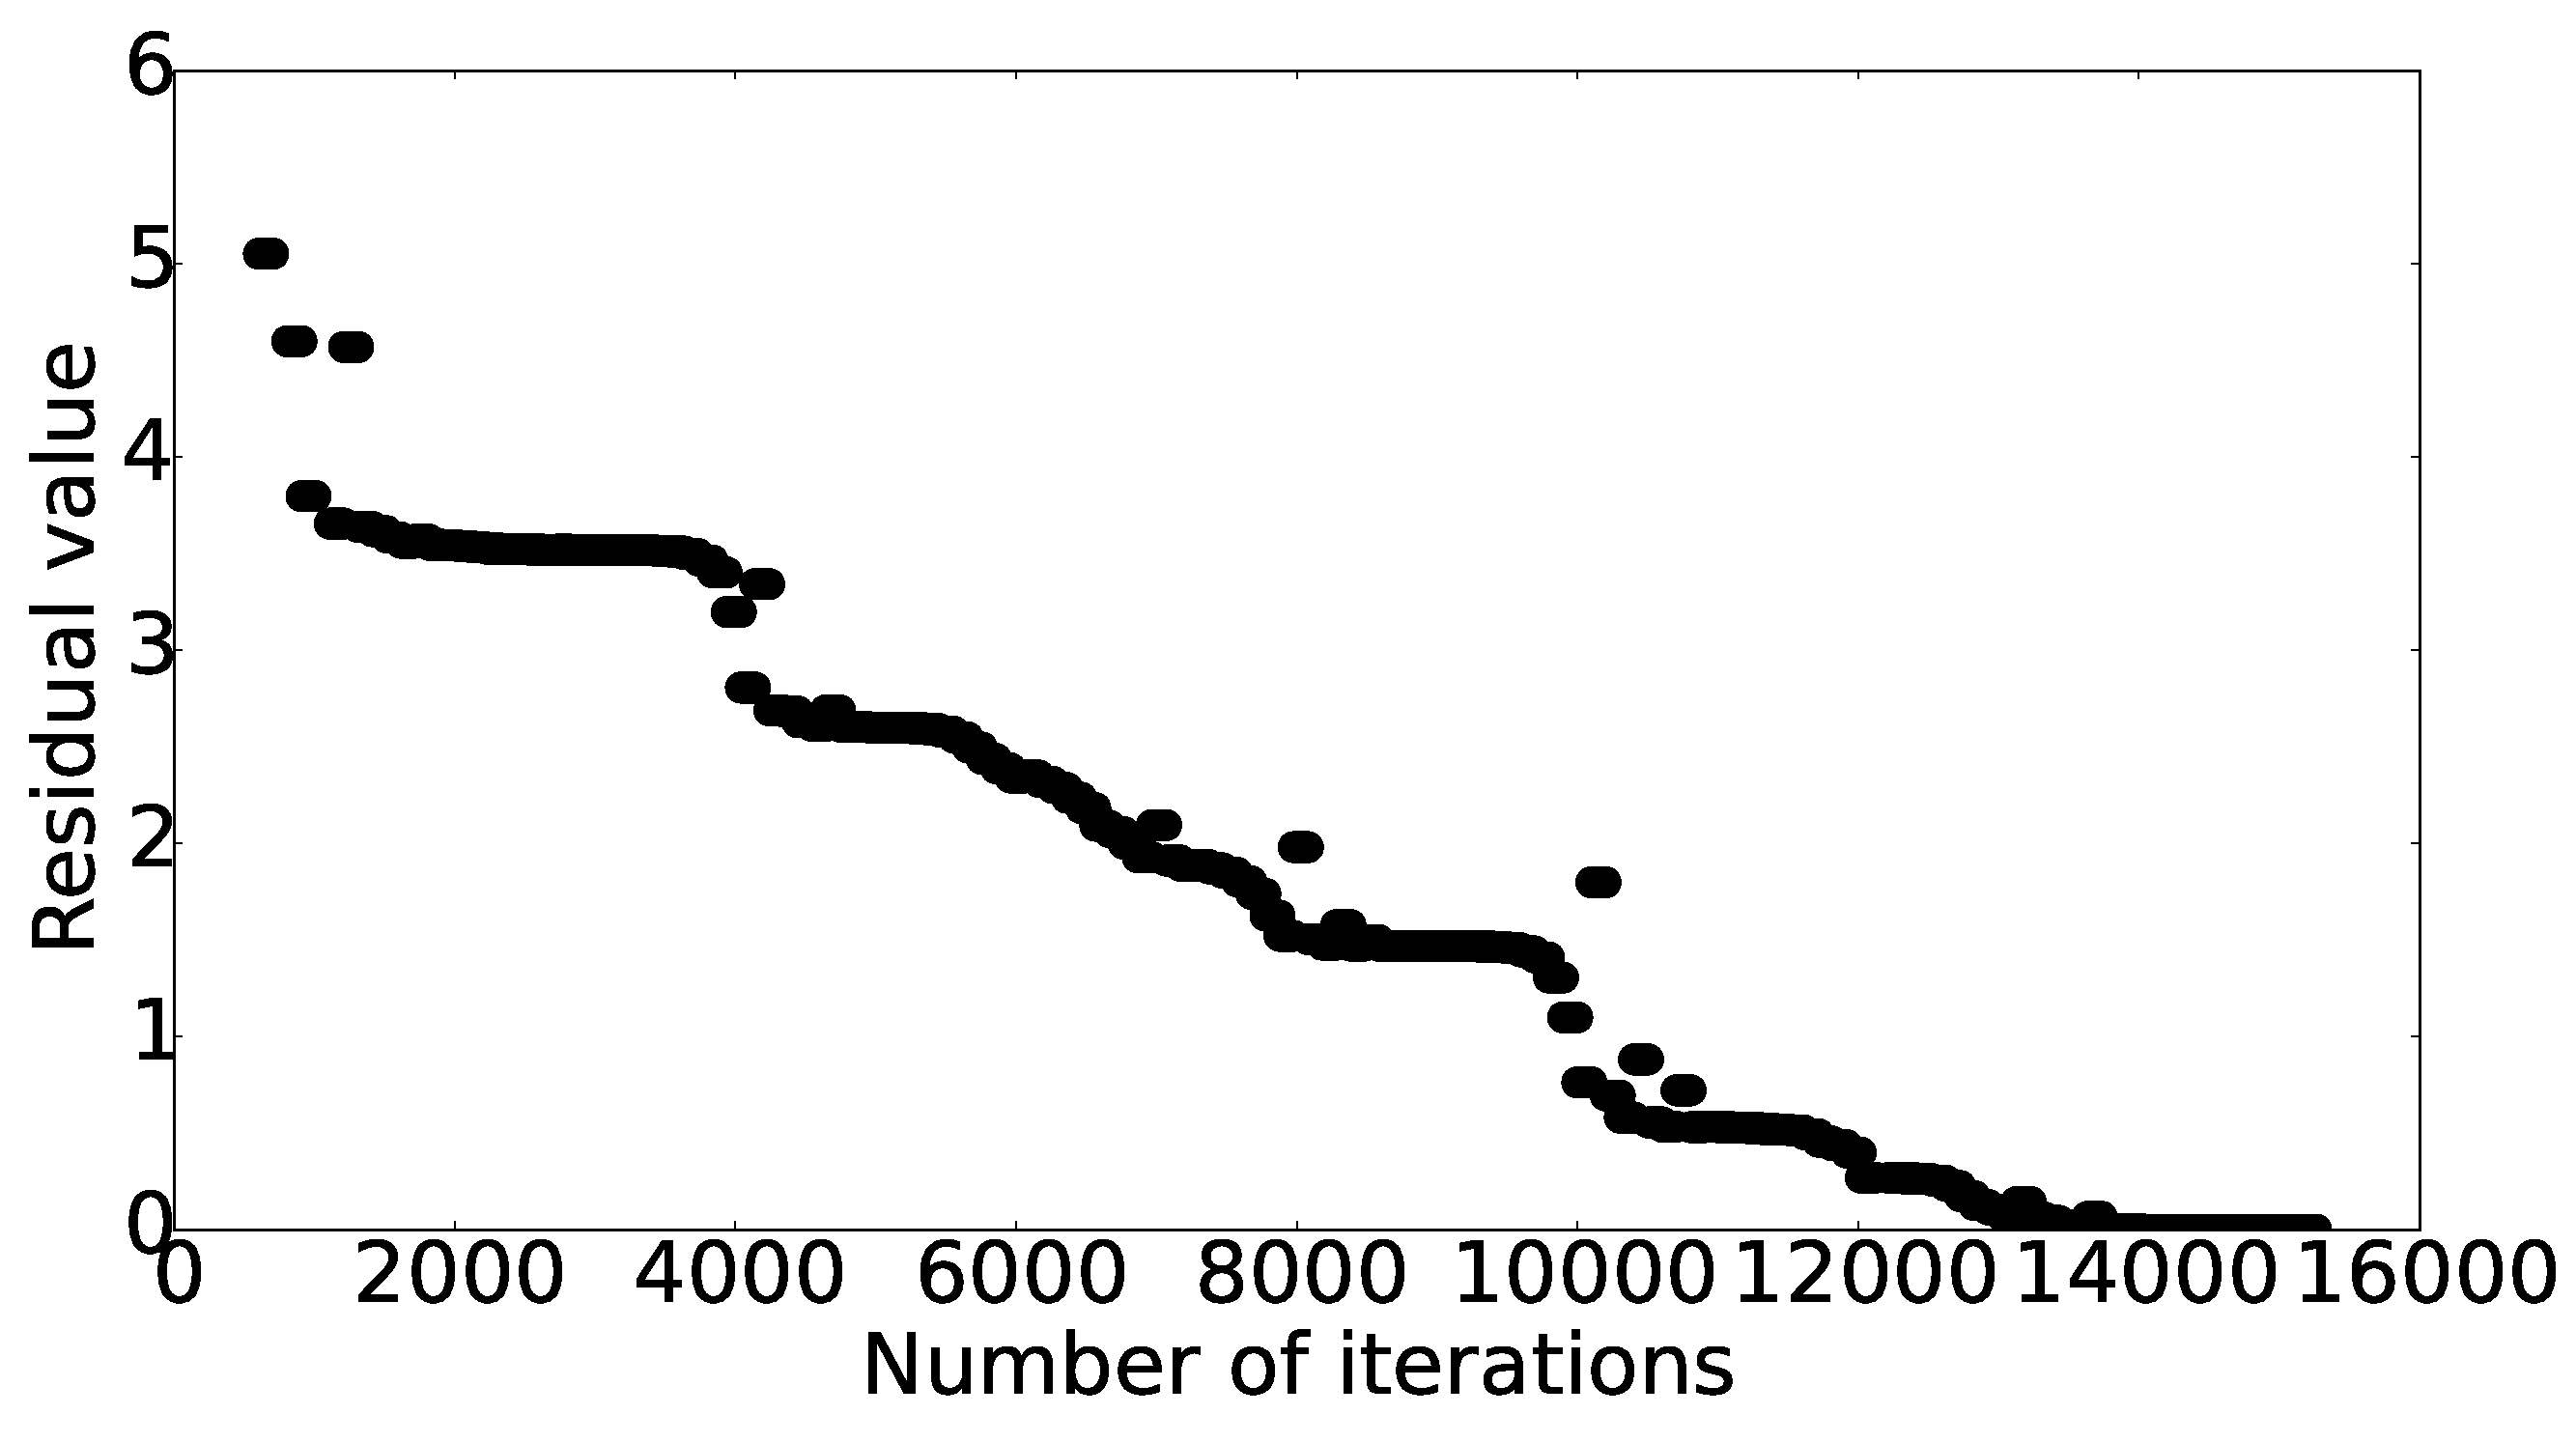
\includegraphics[height=6.00cm]{figure/convergence_study_33.eps}
	\caption{Convergence plot.}
	\label{fig:R3_convergence}
\end{figure}

% -------------------------------------------------------------------
\subsection{Double Pendulum}
Adapting Harmonic balance method for a two-degree of freedom system, a double pendulum, with $\theta_1$ and $\theta_2$ DOF is considered. If $m_1$, $m_2$, $l_1$ and $l_2$,  $c_1$ and $c_2$ are masses, lengths and damping coefficients of pendulum 1 and pendulum 2 respectively, then the equations of motion are
\begin{equation}
(m_1+m_2) l_1 \ddot{\theta_1} + m_2 l_2 \ddot{\theta_2} \cos( \theta_1 - \theta_2 ) + m_2  l_2 \dot{ \theta_2 }^2 \sin( \theta_1 - \theta_2 )+(c_1+c_2) (l_1^2) \dot{\theta_1}+c_2 l_1 l_2  \dot{\theta_2}+ g (m_1+m_2)  \sin( \theta_1) = 0
\end{equation}

\begin{equation}
m_2  l_2 \ddot{\theta_2}+m_2 l_1 \ddot{\theta_1} \cos(\theta_1 - \theta_2)-m_2  l_1 \dot{\theta_1}^2 \sin(\theta_1 - \theta_2)+c_2 \dot{\theta_2}+c_2  l_1  l_2 \dot {\theta_1}+c_2 (l_2^2) \dot{\theta_2}+m_2 g  \sin(\theta_2) = \sin(\omega t)
\end{equation}

The equations of motion are written in state space form 

\begin{equation}
	\dot{u_1} = u_2
\end{equation}

\begin{equation}
	\dot{u_2} = \frac{ed-bf}{ad-bc}	
\end{equation}
\begin{equation}
	\dot{v_1} = v_2 
\end{equation}
\begin{equation}
	\dot{v_2} = \frac{af-ce}{ad-bc}	
\end{equation}

where $a = (m_1+m_2)l_1$, $b= m_2*l_2*cos(u_1-v_1)$, $c=m_2*l_1*cos(u_1-v_1)$, $d = m_2 l_2$, $e= -m_2 l_2 v_2^2 sin(u_1-u_2)-g(m_1+m_2) sin(u_1)+(c_1+c_2) (l_1^2) u_2+c_2 l_1 l_2 v_2$ and $f = m_2 l_1 u_2^2 sin(u_1-v_1)-m_2 g sin(v_1)+ sin(\omega t)+c_2 v2+c_2 l_1 l_2 u_2+c_2 (l_2^2) v_2$


\begin{figure}[H]
	\centering
	\begin{subfigure}[h]{8.0 cm}
		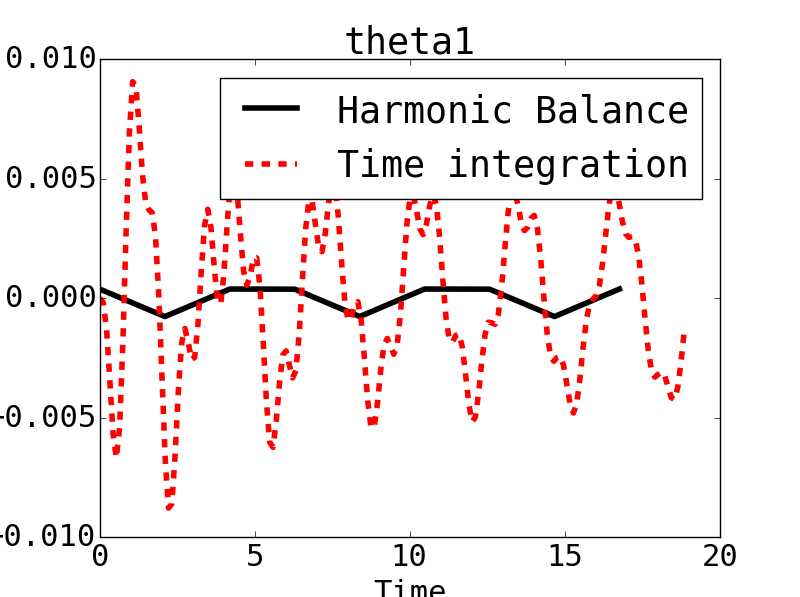
\includegraphics[width=8.0 cm]{figure/p11.png}
		\caption{n = 9}
	\end{subfigure}
	\begin{subfigure}[h]{8.0 cm}
        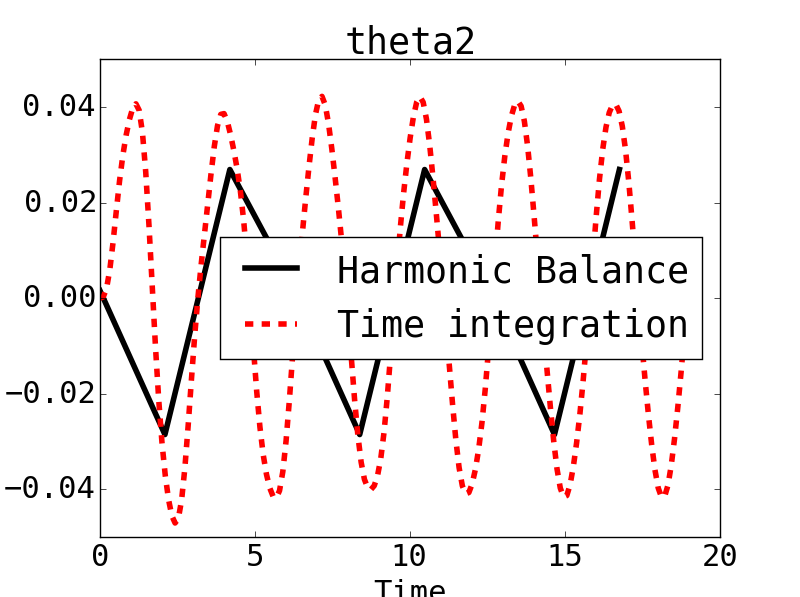
\includegraphics[width=8.0 cm]{figure/p21.png}
		\caption{n = 99}
    \end{subfigure}
    \caption{Comparison between HB and analytical result.}
    \label{fig:Res1}
\end{figure}
\begin{figure}[H]
	\centering
	\begin{subfigure}[h]{8.0 cm}
		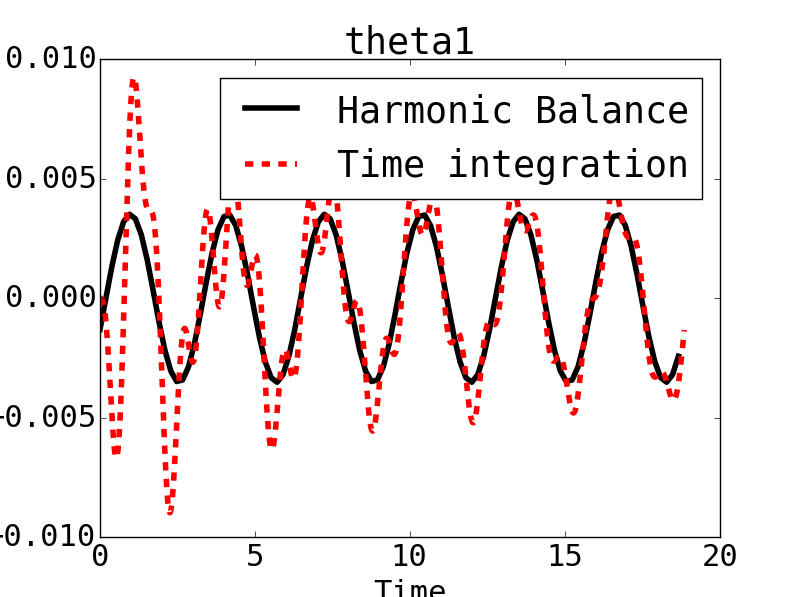
\includegraphics[width=8.0 cm]{figure/p12.png}
		\caption{n = 9}
	\end{subfigure}
	\begin{subfigure}[h]{8.0 cm}
        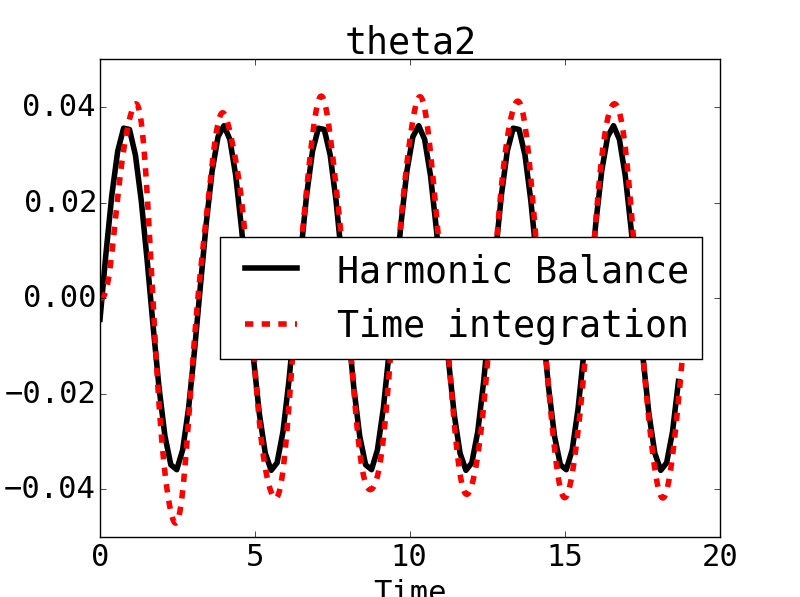
\includegraphics[width=8.0 cm]{figure/p22.png}
		\caption{n = 99}
    \end{subfigure}
    \caption{Comparison between HB and analytical result.}
    \label{fig:Res1}
\end{figure}

The results from Harmonic balance method is in good agreement with the time integrated response for low number and high number of harmonics. 


% -------------------------------------------------------------------
\subsection{Hypersonic Flutter}
In this work, piston theory \cite{ashley2012piston} is applied to a double-wedged lifting surface with pitching degree of freedom as shown in Figure \ref{fig:doubleWedgedAirfoil}. This work uses third-order piston theory to compute unsteady effects behind shock waves and expansion fans and a stiffening spring to the structure. This method of computing unsteady aerodynamic effects delivered highly accurate results when compared to computational fluid dynamics solutions \cite{mcnamara2011aeroelastic}.

\begin{figure}[H]
	\centering
	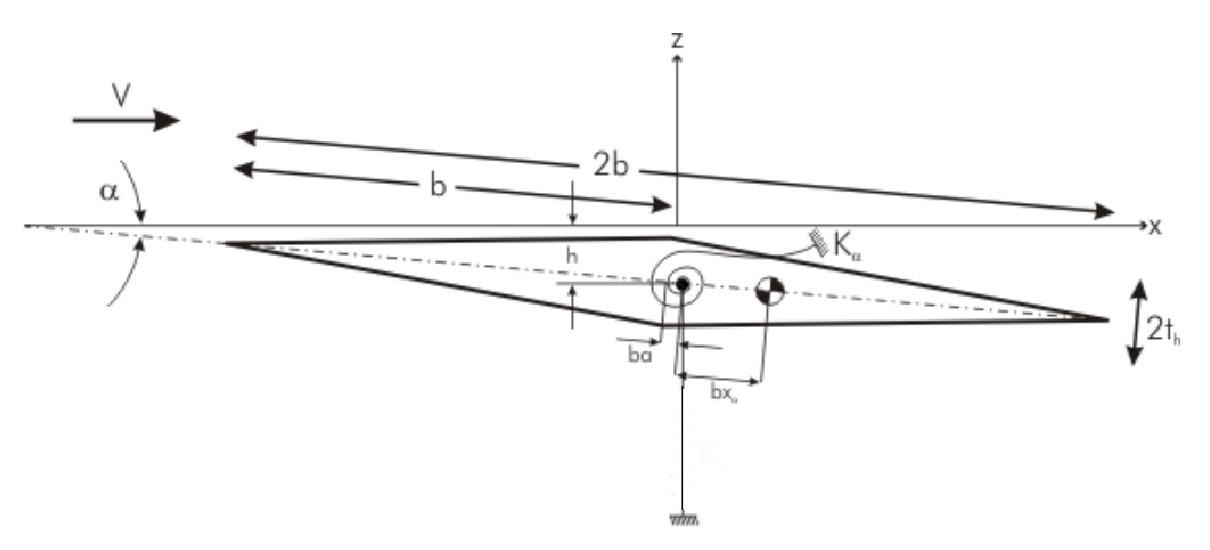
\includegraphics[width=9.00cm]{figure/doubleWedgeAirfoil.png}
	\caption{Double-wedge lifting surface.}
	\label{fig:doubleWedgedAirfoil}
\end{figure}

The governing equation can be written as

\begin{equation}\label{eq:GE}
	m\ddot{\theta} + k \theta = f(\theta, t)
\end{equation}

where $m$ is the mass of airfoil, $k$ is the stiffness, $\theta$ is the angle of attack and $f$ is the aerodynamic load. We use the Piston Theory to calculate the aerodynamic load acting on the airfoil. We used the piston theory to calculate the pressure distribution on the airfoil.

\begin{equation}\label{eq:pistonTheory}
	\frac{P(x, t)}{P_\infty} = \left( 1+ \frac{\gamma - 1}{2} \frac{v_n}{a_\infty} \right)^{\frac{2 \gamma}{\gamma - 1}}
\end{equation}

where $P(x, t)$ is the pressure at point $x$ on the airfoil, $P_\infty$ is the free stream pressure, $\gamma$ is the ratio of specific heats and $a_\infty$ is the speed of sound. The third order expansion of Equation \eqref{eq:pistonTheory} results in

\begin{equation}
	P(x,t) = P_\infty
	\left[
	1 +
	\gamma \frac{v_n}{a_\infty} + 
	\frac{\gamma (\gamma + 1)}{4} \left( \frac{v_n}{a_\infty} \right)^2 + 
	\frac{\gamma (\gamma + 1)}{12} \left( \frac{v_n}{a_\infty} \right)^3
	\right]
\end{equation}

$v_n$ is calculated using the following equation.

\begin{equation}\label{eq:definitionOfVn}
	v_n = \frac{\partial Z(x,t)}{\partial t} + V \frac{\partial Z(x,t)}{\partial x}
\end{equation}

where $V$ is the free stream velocity and $Z(x,t)$ is the position of airfoil surface. The position of airfoil surface can be related to the angle of attack using the following equation:

\begin{equation}\label{eq:definitionOfZ}
	Z(x,t) = M_r\left( \theta(t) \right) Z_0(x)
\end{equation}

where $M_r$ is the rotation matrix, and $Z_0(x)$ is the initial shape of the airfoil.  As can be seen here, the location of surface at time $t$ only depends on the angle of attach at that time, $\theta(t)$. The rotation matrix is defined as

\begin{equation*}
	M_r = 
	\begin{bmatrix}
		\cos \theta & -\sin \theta \\
		\sin \theta & \cos \theta
	\end{bmatrix}
\end{equation*}

By expanding Equation \eqref{eq:pistonTheory}, and substituting for $Z(x,t)$ from Equation \eqref{eq:definitionOfZ}, Equation \eqref{eq:GE} can be rewritten as

\begin{subequations}
\begin{gather}
	m\ddot{\theta} + k \theta = 
	\oint_{airfoil} P_\infty
	\left[
	\gamma \frac{v_n}{a_\infty} +
	\frac{\gamma (\gamma + 1)}{4} \left( \frac{v_n}{a_\infty}\right)^2 +
	1
	\right] ds
	\\
	v_n = 
	\frac{\partial M_r(\theta)}{\partial t}Z_0(x) + V M_r(\theta)\frac{\partial Z_0(x)}{\partial x}
\end{gather}\label{eq:GEfull}
\end{subequations}

Equation \eqref{eq:GEfull} needs to be solved for $\theta$ using Harmonic Balance method. For this problem the operating conditions of the vehicle are selected as follows:

\begin{table}[htbp]
\begin{center}
\begin{tabular}{c|c}
	$\gamma$ & 1.4 \\ \hline
	$a_\infty$ & 343 m/s \\ \hline
	$P_\infty$ & 10 Pa \\ \hline
	V & 600 m/s \\
	\end{tabular}
	\end{center}
	\caption{Operating conditions.}
\end{table}

For verification, the harmonic balance results are compared with the numerical integration is Figure \eqref{fig:hypersonicFlutterResult}. As shown here, the harmonic balance predicts a static solution ($\theta(t_\infty) = -1.706$) however, the numerical integration predicts oscillation. The interesting point in here is that the time average value of numerical integration is the same as harmonic balance results. This means that the harmonic balance did not have enough frequency content to capture the oscillations. It only captured the constant term.

\begin{figure}[H]
	\centering
	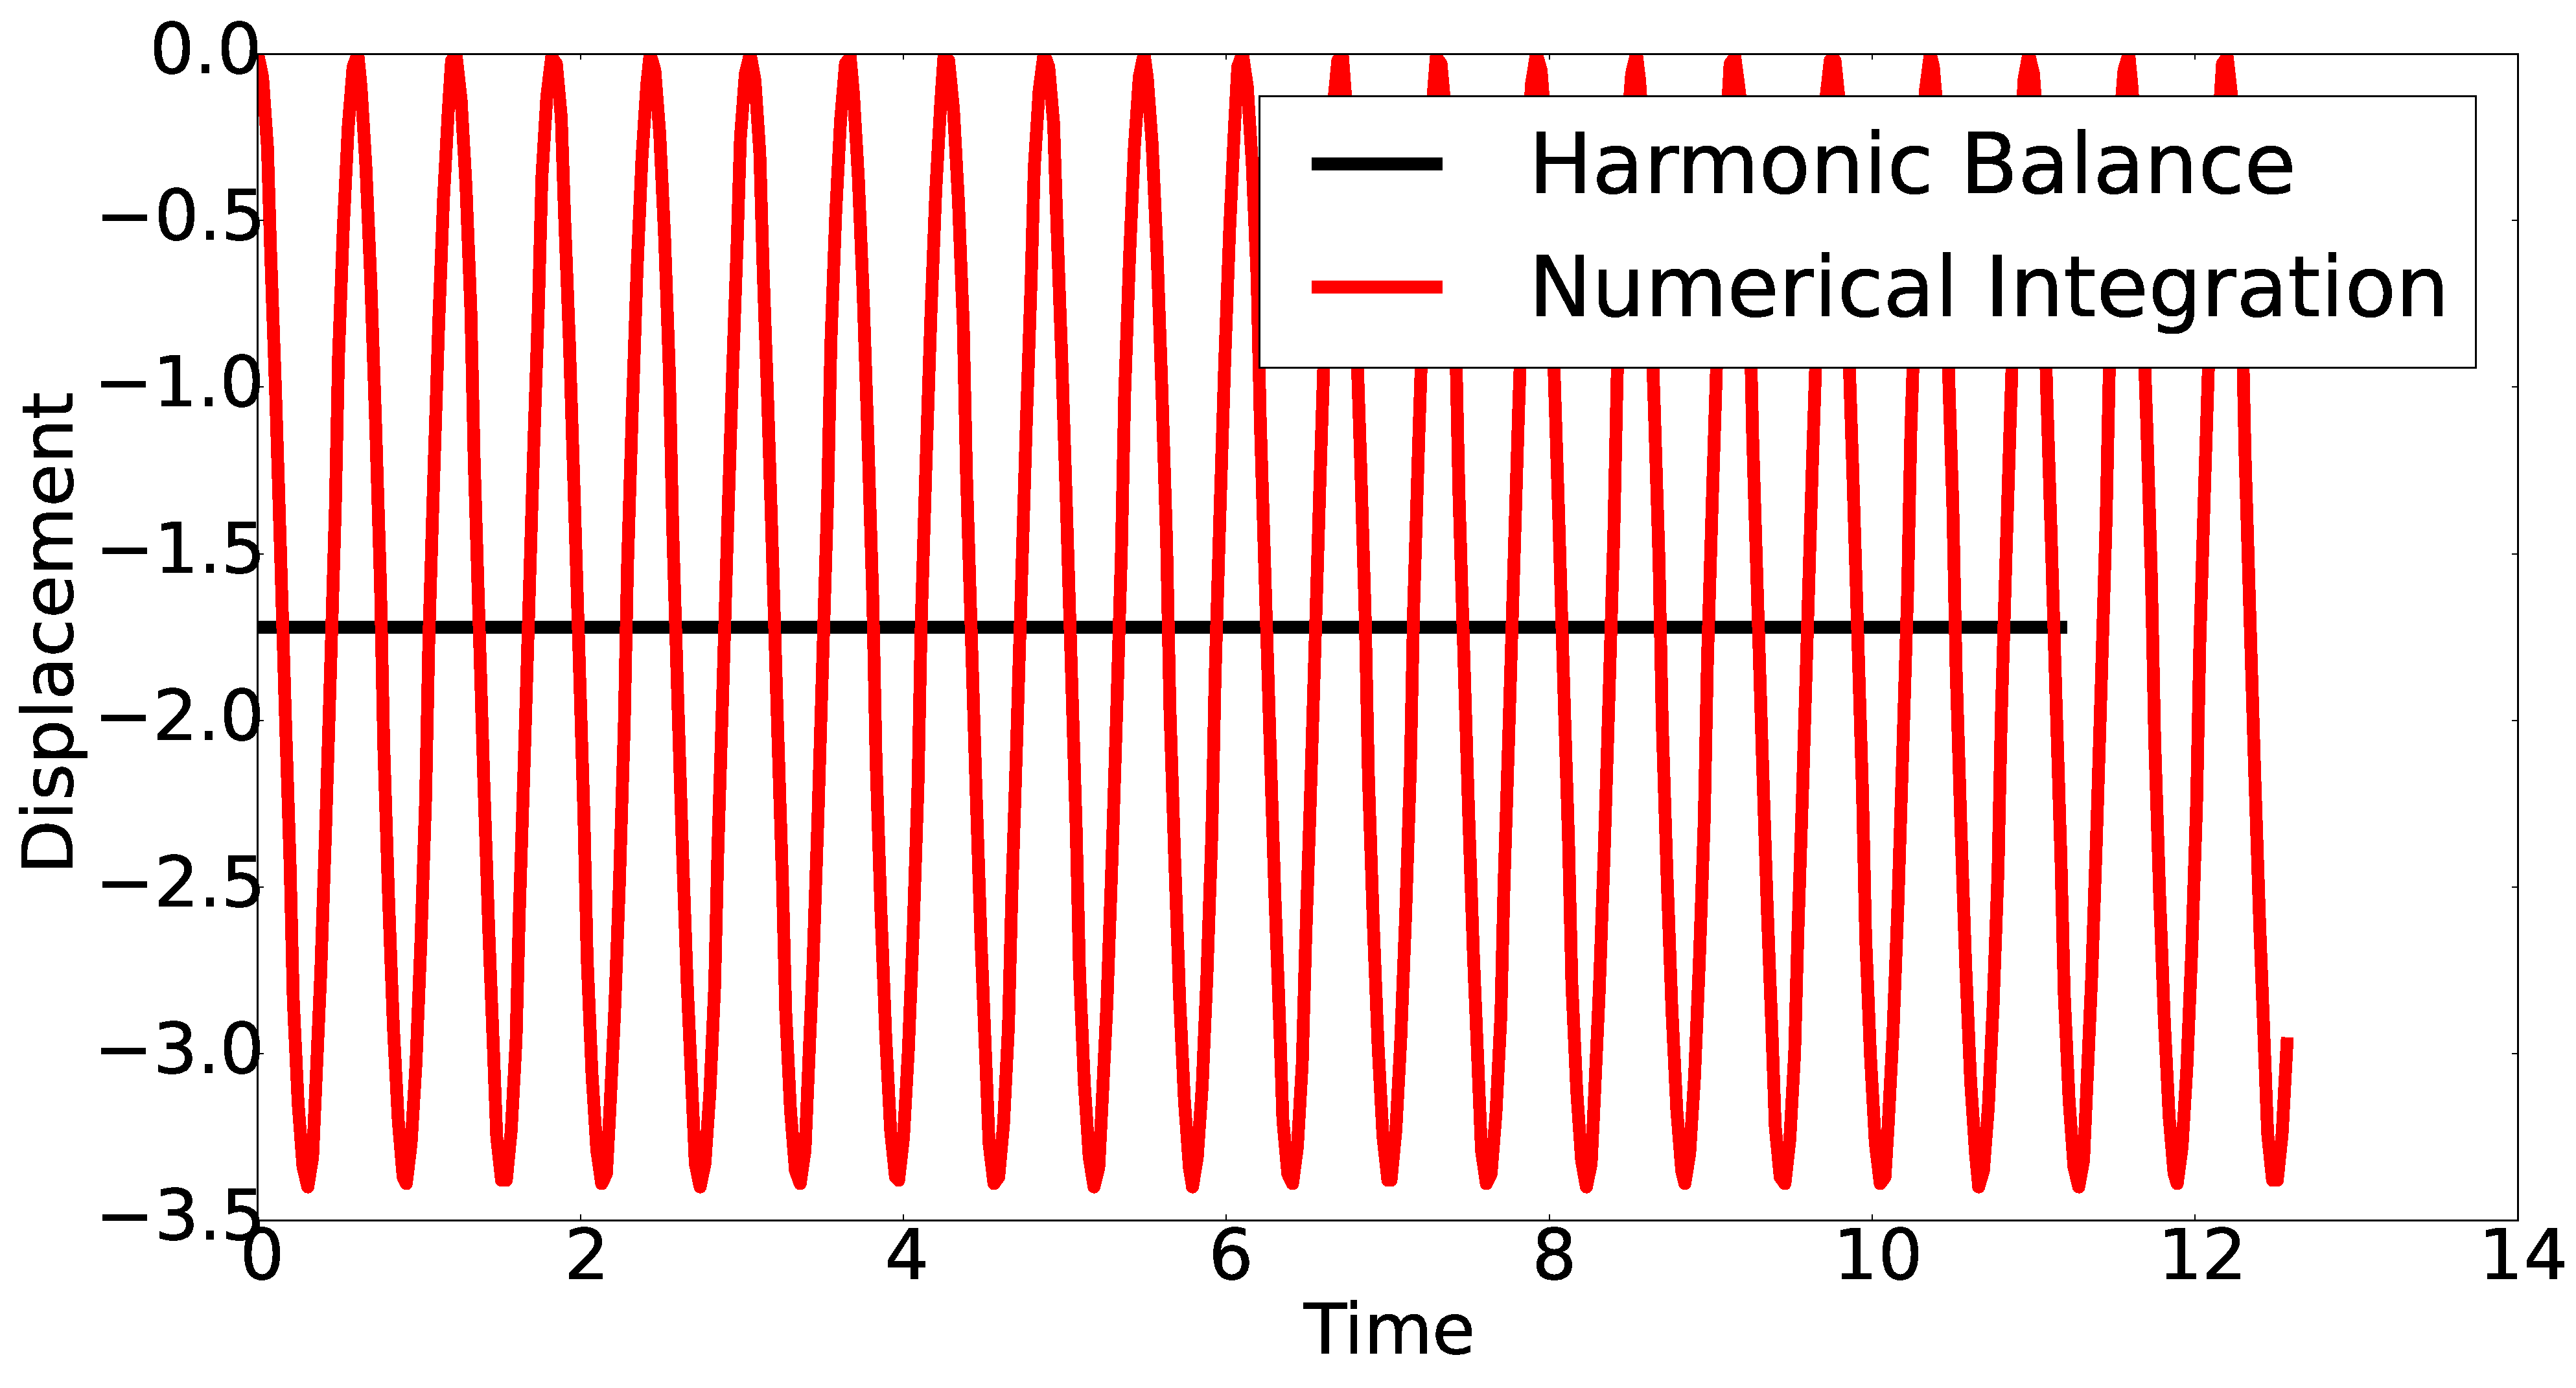
\includegraphics[width=12.0 cm]{figure/4N9.eps}
	\caption{Comparison between HB and analytical result}
	\label{fig:hypersonicFlutterResult}
\end{figure}

\section{Conclusions}

In this project, Harmonic balance method is applied to linear and non-linear equations. The results are compared with the time-integrated responses of these systems. Initially, linear system is solved to validate the results from Harmonic Balance method and time integrated methods and the study is extended to non-linear systems like two-dof system, parametrically oscillated system and systems with flutter responses. 

Responses from linear and moderately non-linear systems using Harmonic Balance method converge to the time-integrated response in due course of time. This is because Harmonic balance method results in steady-state reponse and it is required to let the transient response of the time integration to die of before comparing the results. Taking more frequency components into account, Harmonic Balance Method provides better approximation to the response. 

Overall, Harmonic balance method is efficient in obtaining closed form steady-state solution to the non-linear equations.

% ===================================================================
\newpage
\section{Appendices}
\lstinputlisting{code/31.py}
\newpage
\lstinputlisting{code/32.py}
\newpage
\lstinputlisting{code/33.py}
\newpage
\lstinputlisting{code/34.py}
\newpage
\lstinputlisting{code/35.py}
\newpage
\lstinputlisting{code/Pendulum.py}
\newpage
\lstinputlisting{code/aerodynamic.py}
\newpage
\lstinputlisting{code/samyukta.m}
\newpage
\lstinputlisting{code/getShape.py}
\newpage
\bibliographystyle{aiaa}
\bibliography{ref}
\end{document}
